%%------------------ paramètres préliminaires-------------- 


%%---chargement des packages

\documentclass[10pt,a4paper]{report} % commande de classe avec des arguments {obligatoire} et [optionnels]

\usepackage[T1]{fontenc}              % encodage des fontes
\usepackage[utf8]{inputenc}           % encodage des fichiers
\usepackage[french]{babel}  % traduction en français des en-tetes de parties et chapitre
\usepackage{parskip} %centrage et mise en page, utilisé pour la page de titre
\usepackage{graphicx} %pour ajouter des images
\usepackage{appendix} %gestion des annexes
\usepackage{pdfpages} %pour ajouter un pdf au doc
\usepackage{subcaption}

\usepackage[
   backend=biber,        % compilateur par défaut pour biblatex
   sorting=nyt,          % trier par nom, année, titre
   citestyle=authoryear, % style de citation auteur-année
   bibstyle=authoryear,  % style de bibliographie alphabétique
]{biblatex}

\addbibresource{BIBLIO_rapport-de-stage.bib} %bibliographie à utiliser

%%---redéfinition de fonctions

\newcommand{\mychapter}[2]{ %rédapatation de la numérotation des chapitres
    \setcounter{chapter}{#1}
    \setcounter{section}{0}
    \chapter*{#2}
    \addcontentsline{toc}{chapter}{#2}
}

\renewcommand{\appendixpagename}{Annexes} %change le résultat affiché par une commande, ici pour avoir le résultat en français
\renewcommand{\appendixtocname}{Annexes}


%%---------------------------------------------------------------
%%------------------------corps du document----------------------
%%---------------------------------------------------------------


\begin{document}

%%------------------ TITRE -------------------------------

%%Variables du document
\title{Cartographie en gestion de crise}
\author{Cyprien Deloget}
\date{2021-2022}

%\maketitle %Afficage du titre dans lequel on verra les 3 variables au dessus
\begin{titlepage}
    \begin{center}
        \vspace*{0.25cm}
        Rapport de stage\\
        \vspace{0.5cm}
        \textbf{\huge Cartographie en gestion de crise}
 
        \vspace{0.5cm}
        Institut des Hautes Études du Ministère de l'Intérieur \\
        (IHEMI)
        \vspace{0.5cm}
 
        \textbf{Cyprien DELOGET}
        \vspace{1cm}

        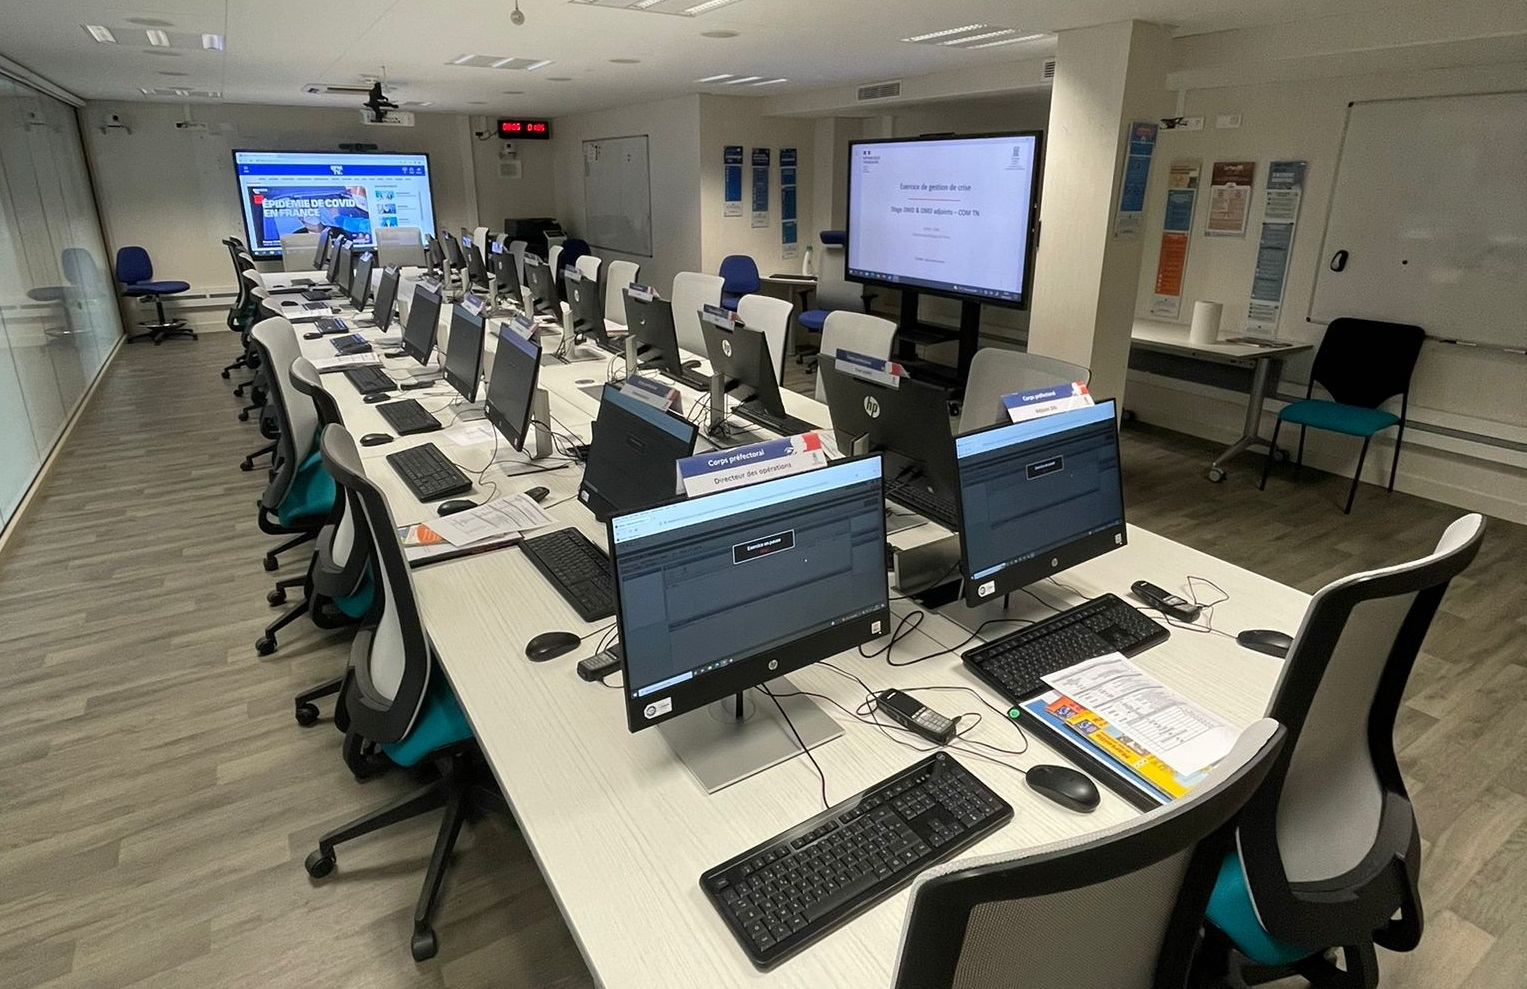
\includegraphics[width = 0.95\textwidth]{salledecrise_titlepage.jpg}
        \vfill
        \vspace{1cm}
        Tutrice : Mme Anne-Lise Coeur-Bizot\\
        Encadrant universitaire : M. Adrien Van Hamme\\
        \vspace{0.25cm}    
        Master 2 Carthagéo\\
        2021 - 2022
        
        \vspace{0.6cm}

        \begin{minipage}{0.3\textwidth}
            \centering
            
\includegraphics[width=.6\linewidth]{ensg.png}
        \end{minipage}\hfill
        \begin{minipage}{0.3\textwidth}
            \centering
            
\includegraphics[width=.7\linewidth]{pariscite.jpg}
        \end{minipage}
        \begin{minipage}{0.3\textwidth}
            \centering
            
\includegraphics[width=.7\linewidth]{sorbonne.png}
        \end{minipage}

             
    \end{center}
 \end{titlepage}

\newpage
\thispagestyle{empty}
\mbox{}
\newpage

%%------------------- RESUME ---------------------

\begin{abstract}
    Ce rapport de stage fait suite à la réalisation d’un stage en tant que cartographe au sein de l’Institut des Hautes Études du ministère de l’intérieur (IHEMI). Il présente les missions de l’un de ses départements, le Département Risque et Crise dans lequel s’est déroulé le stage. Ce travail se focalise sur la formation à la gestion de crise assurée par le DRC. Structuré autour d’une présentation non exhaustive de ce qu’est la gestion de crises en France, il a pour objectif de montrer, tout en présentant les résultats des demandes formulées, comment et via quelles particularités la réalisation de cartes s’intègre dans la gestion de crise en tant qu’ensemble de procédés. 
    
    C’est aussi un support de réflexions sur la place d’un cartographe dans ce champ professionnel mais aussi une tentative de bilan personnel de fin d’études.
\end{abstract}


\tableofcontents{}

\newpage
\thispagestyle{empty}
\mbox{}
\newpage


%%---------------------INTRO-------------------------

\part*{Introduction}

La rédaction de ce document s’inscrit dans le cadre de la réalisation de mon stage de fin d’études du Master Carthagéo. Celui-ci s’est déroulé au sein de l’Institut des Hautes Études du ministère de l’Intérieur (IHEMI), au sein d’une équipe spécialisée dans la formation à la gestion de crise. J’y ai, pendant cinq mois, occupé le poste de cartographe. 

Dans de cadre-ci, plusieurs missions m’ont été confiées. Ce rapport n’est toutefois pas structuré autour de celles-ci. Les évoquer indépendamment les unes des autres et de manière peu reliée au contexte de déroulement du stage n’aurait que peu d’intérêt. C’est pourquoi les chapitres de ce rapport ont été établis en fonction du niveau d’analyse et de détail abordé, à la fois dans la présentation du contexte et des modalités du stage que dans les missions et réalisations cartographiques qui m’ont été demandées. C’est pourquoi un même aspect pourra être abordé dans plusieurs parties de ce rapport, mais à chaque fois sous un angle différent et avec un propos différent. De ce fait, un chapitre s’appuiera souvent sur des éléments listés dans le chapitre précédent pour en détailler certains aspects sous un autre angle.

 Une première partie de ce rapport consistera à présenter l’organisation, les missions et l’environnement institutionnel de l’IHEMI. Tout d’abord, son organisation et son fonctionnement de manière générale. Nous montrerons la particularité de son positionnement interministériel et de sa transversalité et ce bien qu’il soit rattaché au ministère de l’Intérieur. Ensuite, nous présenterons les missions et l’organisation du Département Risques et Crises (DRC). 

La seconde partie, centrale dans ce rapport, est dédiée à la présentation de la gestion de crise et à la manière dont s’y intègrent des besoins en cartographie préalables à mes missions. En donner une définition est essentiel pour ensuite comprendre comment la réalisation de cartes s’y intègre. Nous verrons à la fois la gestion de crise dans son volet essentiellement institutionnel, dans la sphère publique. La gestion de crises se fait aussi par des acteurs privés. Notre attention se portera notamment sur la dimension pédagogique, avec la formation pratique à la gestion de crise, qui est la principale mission du DRC. Nous détaillerons les points enseignés par le DRC, ainsi que le public reçu et le public ciblé, ainsi que le cadre et les outils dont il dispose pour mener ses formations. La dernière partie consistera en un recul critique sur les réalisations, ainsi qu’une proposition d’améliorations et de réflexions plus globales. Là où la seconde partie portera sur des cas pratiques et concrets tirés du déroulement de mon stage, cette dernière partie consistera en une vision portant sur la cartographie en général, les points d’attention, les limites et pièges que j’aurai tenté d’identifier. Elle servira toutefois de cadre pour présenter certaines de mes réalisations.

Les missions à proprement parler seront abordées dans ce cadre-ci, mêlées dans les parties et sous parties décrites ci-dessus, de la manière la plus claire possible. Précisons toutefois d’avance, par soucis de clarté, que mes missions relèvent d’un point de vue technique de trois différents types de réalisation, dont le temps consacré à chacune est détaillé en annexe 1 : 


\begin{itemize}
    \item Cartes éditoriales sous logiciel SIG et logiciel DAO
    \item Réalisation de cartes lors d’exercices de gestion de crise
    \item Conception et début de réalisation d’une application web
\end{itemize}

Ce rapport ne se veut donc pas seulement un compte rendu de mes missions et réalisations, mais bel et bien une entrée en matière dans la formation à la gestion de crise dans une structure publique interprofessionnelle et surtout une tentative d’identifier les particularités des réalisations cartographiques dans ce contexte.

Ce rapport rend compte d’un stage dans un milieu professionnel spécifique. Il se veut toutefois accessible à un grand public curieux. Ainsi, une attention est portée au fait de détailler chaque acronyme lors de sa première apparition. Cela n’est toutefois pas le cas pour certains d’entre eux par soucis d’une plus grande fluidité de lecture. Néanmoins, un glossaire est présent en fin de document.



\newpage
\thispagestyle{empty}
\mbox{}
\newpage

%%---------------------------------PREMIERE PARTIE--------------------------------------

\begin{part}{L’institut des Hautes Études du ministère de l’Intérieur : son statut, ses interlocuteurs, ses missions}

Ce premier chapitre détaille ses spécificités, tout en présentant la structure générale dans laquelle j’évolue durant mon stage. La première sous-partie propose ainsi d’expliquer ces mêmes spécificités. D’abord à l’échelle de l’Institut, après une explication de son positionnement qui est en partie lié à son histoire. Nous présenterons ensuite son organisation interne. La seconde sous-partie est consacrée à la composition et aux missions du DRC et à son fonctionnement, composé de sept agents titulaires et de trois stagiaires ou alternants. Il s’agira ici d’en montrer les spécificités cette fois-ci internes, vis-à-vis des autres départements.

\mychapter{0}{Un service de ministère de l’Intérieur aux multiples interlocuteurs}


L’IHEMI a été créé en 2020 et résulte de la fusion du Centre des Hautes Études du ministère de l’Intérieur (CHEMI) et de l’Institut National des Hautes Etudes de Sécurité et Justice (INHESJ). Ce dernier était rattaché aux Services du Premier Ministre, ce qui instituait donc, déjà, un statut interministériel.

Le CHEMI ayant pour mission la « formation des hauts cadres civils et militaires du Ministère », il s’agissait d’un organisme de formation interne au Ministère de l’Intérieur, organisant notamment des Journées d’Études et de Réflexion (JER). L’INHESJ était quant à lui un établissement d’enseignement supérieur composé « d’un comité scientifique et assurant plusieurs sessions nationales annuelles » de formations sur les thèmes suivants : Sécurité et Justice ; Management Stratégique de la Crise ; Protection des entreprise et Intelligence économique. \footcite{Decret20091321282009}

L’IHEMI reprend les missions et compétences de ces structures, dans les locaux de l’INHESJ, situés au sein de l’Ecole Militaire, dans le 7e arrondissement de Paris. L’IHEMI conserve également, en site annexe, les bureaux du CHEMI, situés dans le Fort de Charenton à Maisons-Alfort (site appartenant à la Gendarmerie). L’Ecole Militaire est, comme son nom l’indique, un site militaire. L’IHEMI est la seule structure de l’Ecole Militaire qui ne dépend pas du ministère des Armées et qui est donc sous statut civil.

La mission de l’IHEMI est double : un volet recherche sur les mêmes thématiques de la crise et de la sécurité (globalement les missions portées par le ministère de l’Intérieur) et un volet formation, notamment au travers des trois sessions nationales d’une durée d’un an, à la fois pour un public de fonctionnaires des ministères, et à la fois vers un public extérieur. Une troisième mission s’ajoute : la diffusion de la connaissance, au travers d’une lettre d’information et de la publication de revues. \cite{ihemiOrganisationIHEMI}

Un organisme semblable, de création plus ancienne et qui a inspiré le fonctionnement de l’IHEMI, existe pour le ministère des Armées : il s’agit de l’IHEDN.


L’IHEMI se compose d’une direction et d’un secrétariat général. Sa direction est assurée par un préfet. Ce dernier \footnote{Il s’agit au moment où j’écris ce rapport de M. Éric Freysselinard, qui a notamment occupé les postes de préfet de l’Aude et de Meurthe-et-Moselle}  est par définition nommé en Conseil des Ministres. L’IHEMI est donc, de fait, considéré comme un service dépendant du ministère de l’Intérieur, où son préfet est directement placé sous l’autorité du Ministre. Il ne dispose pas, à ce titre, d’assemblée délibérante fixant ses orientations, comme cela est le cas pour un Établissement Public par exemple.

Du fait de cette dépendance hiérarchique, l’IHEMI peut aussi dans certains cas, utiliser des locaux situés place Beauvau ou à Lognes dans les locaux de la Sous-Direction du Recrutement et de la Formation (SDRF). La figure ~\ref{fig1} ci-dessous présente les sites liés à l’IHEMI
%figure 1
\begin{figure}[!t]
    \centering
    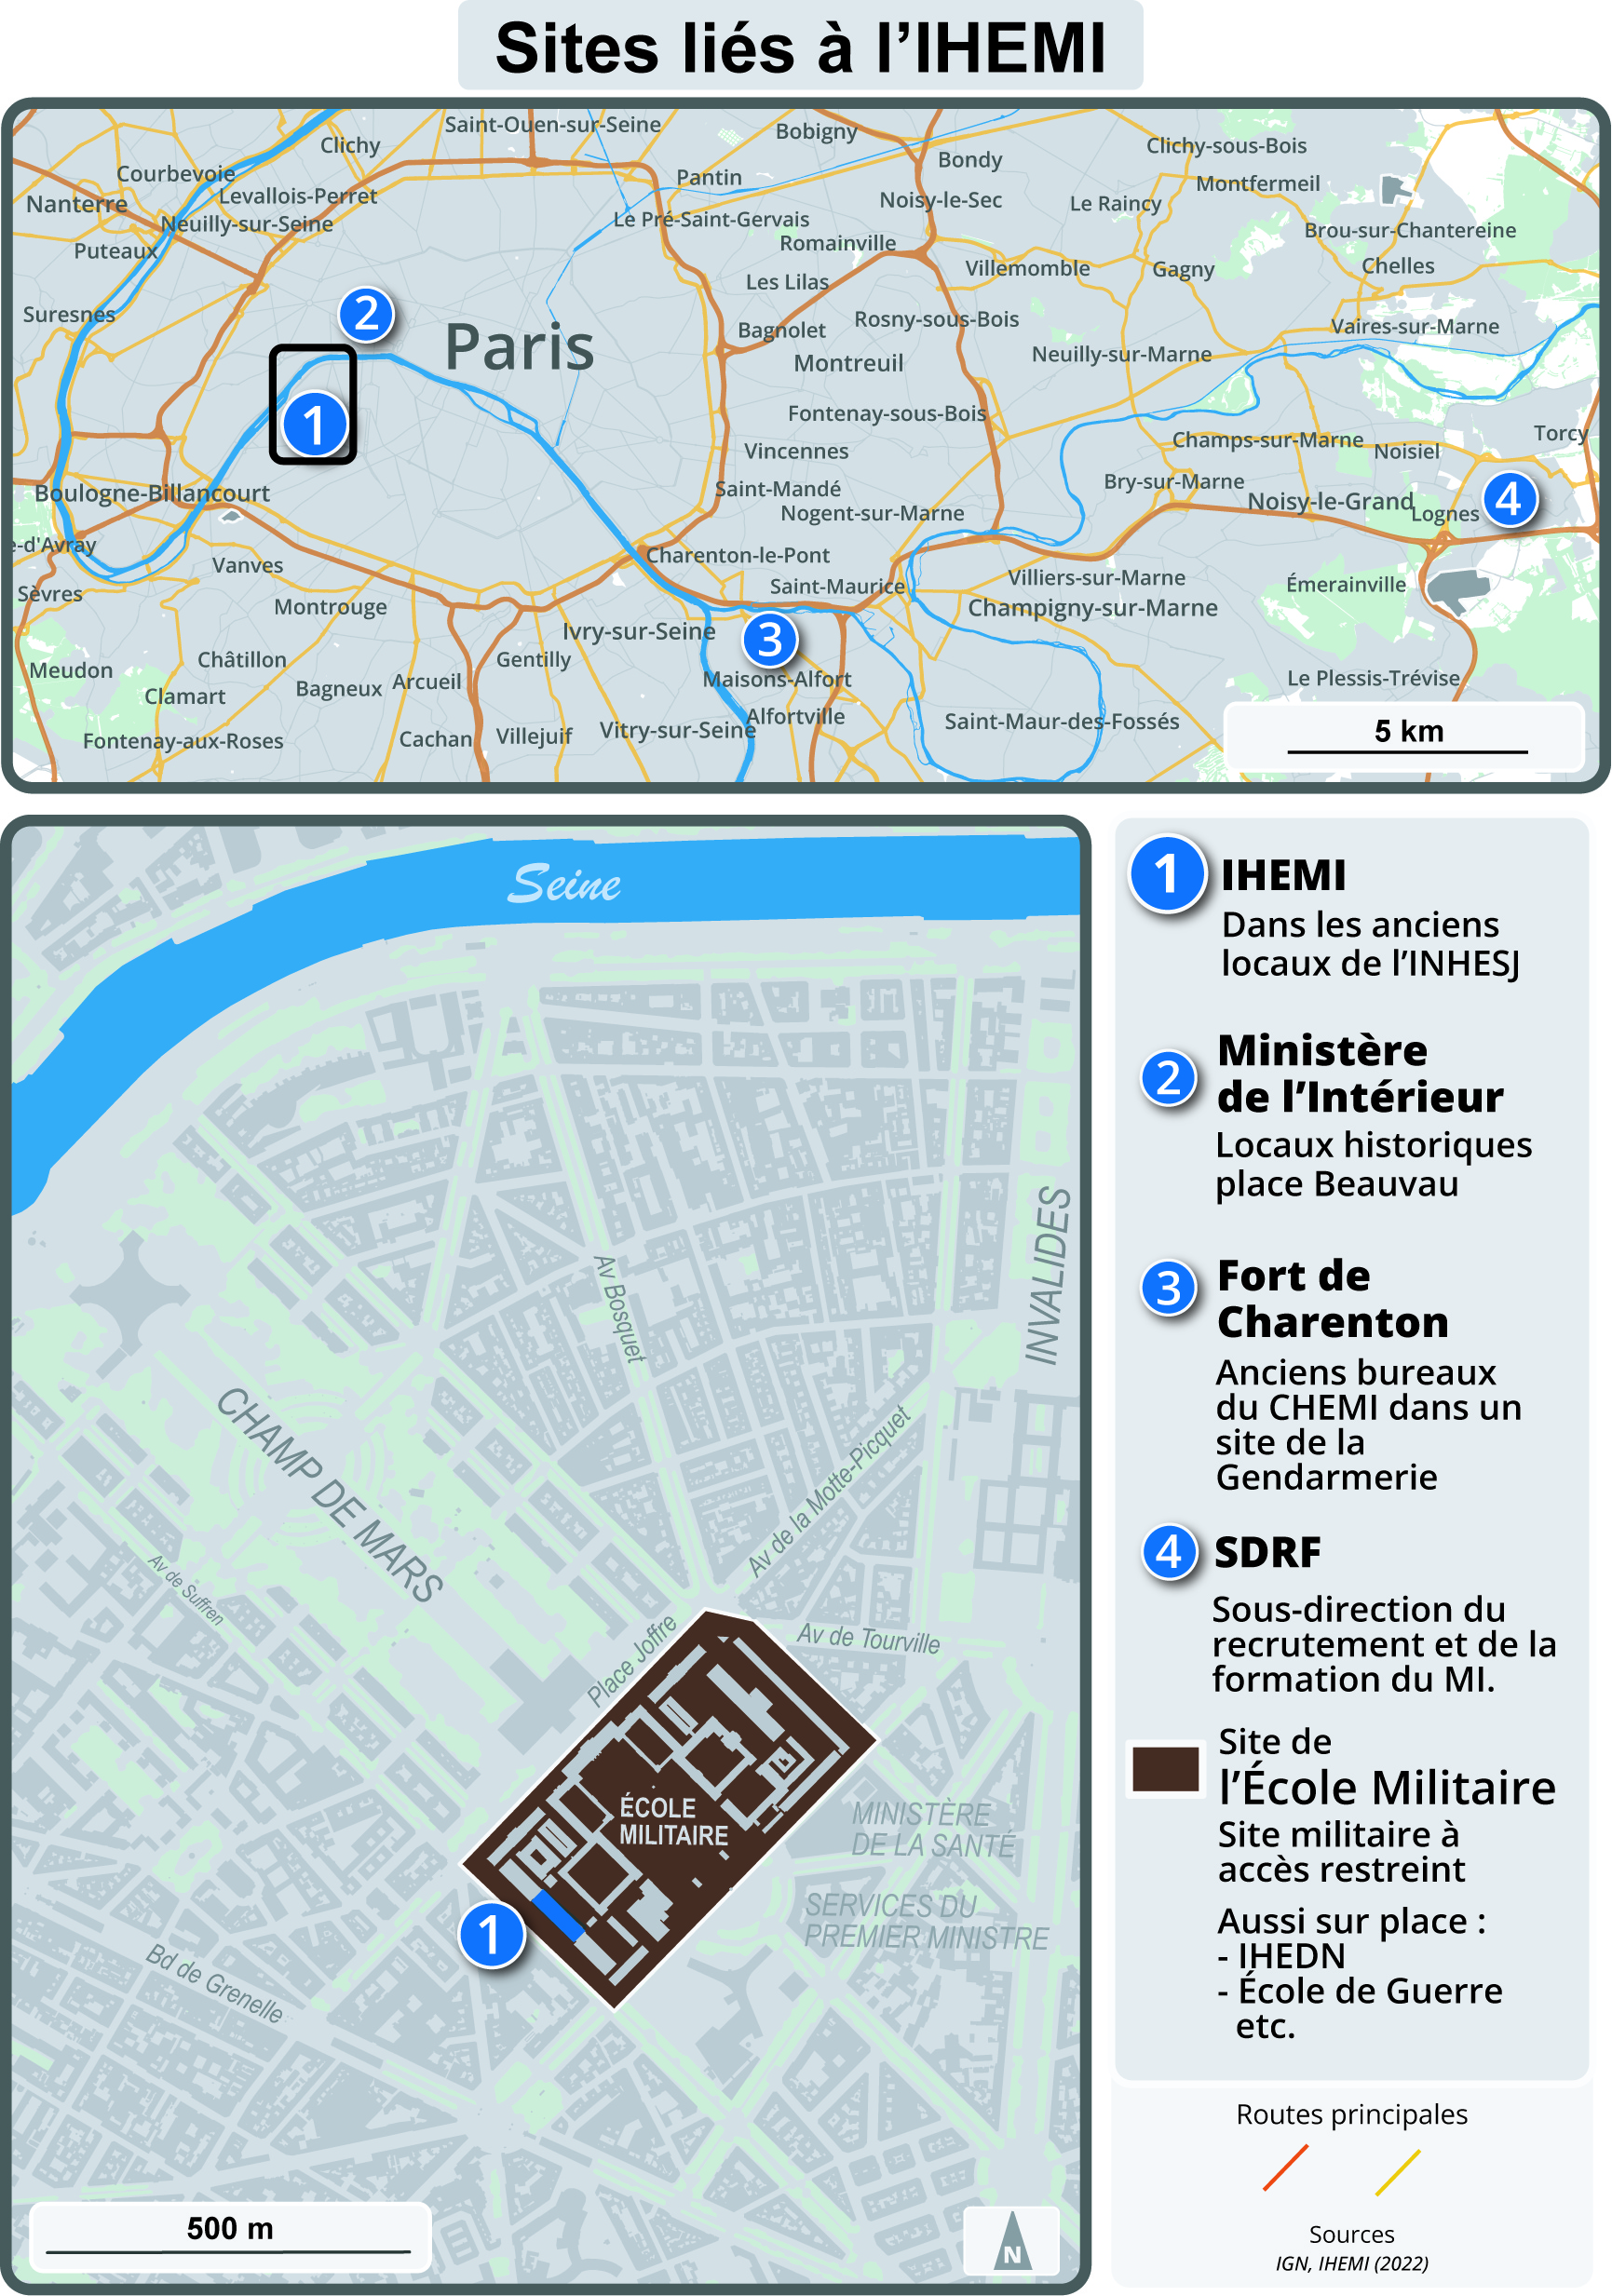
\includegraphics[width=0.95\textwidth]{figures/carte_situ.jpg}
    \caption{Présentation des différentes sites liés à l’IHEMI et utilisés par celui-ci en région parisienne ; source : personnel}
    \label{fig1}
\end{figure}

Outre une Direction des Cycles et des Etudes composée d’un département Sécurité et Justice (qui gère la session nationale éponyme) et d’un département formation qui « reprend les produits hérités du CHEMI », L’IHEMI se compose également d’une direction Recherche et Prospective et d’une Direction de la Stratégie des Risques et des Relations Internationales (DSRI). 

Cette DSRI, à laquelle j’étais rattachée, se compose de plusieurs départements :
\begin{itemize}
    \item Rayonnement International, qui prend en charge les formations liées notamment aux institutions européennes et à la Présidence Française de l’Union Européenne (PFUE)
    \item Réflexion Stratégique, qui reprend les JER au profit du ministère de l’Intérieur et organise également le Cycle des Hautes Etudes Territoriales, qui est une session de formation au profit d’auditeurs extérieurs au ministère de l’Intérieur ayant pour vocation à occuper des fonctions de préfet.
\end{itemize}

Les deux départements suivants sont, en termes d’effectifs, les plus importants

\begin{itemize}
    \item Intelligence et Sécurité Economique (dit « IE »), plus ancienne entité de l’IHEMI, crée en 1997 sous forme d’une collaboration entre la Gendarmerie et le Club de Sécurité des Entreprises. Ce département pilote la Sessions nationale Protection des Entreprises et Sécurité Economique.
    \item Risques et Crises (dit « DRC ») : organise des formations en gestion des crises à destination des organismes, historiquement publics mais surtout privés, au niveau national, avec des sessions de formations allant d’une demi-journée à plusieurs jours. La plupart des formations sont dispensées sur le site de l’IHEMI par nécessité technique. Le DRC est en effet le seul département à disposer de plateaux techniques dédiés aux formations qu’il assure. L’équipe se déplace également en région lorsque nécessaire. Le DRC pilote également une session nationale « Management Stratégique de la Crise » (dite « SNC »), formation sélective d’une durée d’un an, reconnue au RNCP et délivrant l’équivalent d’un Master 2.
\end{itemize}

L’ensemble de ces départements a pour missions, notamment, de dispenser des sessions de formations. Celles-ci sont dispensées par ses effectifs, pourvus par des chargés de missions et des fonctionnaires détachés d’autres services ou d’autres ministères. Lorsque la spécificité d’une formation le requiert, des intervenants extérieurs sont mobilisés, contre rémunération ou à titre gratuit. Ils sont souvent issus de la sphère professionnelle de l’administration publique, et peuvent eux-mêmes avoir une expérience dans un autre service du ministère de l’intérieur ou d’un autre ministère. Cette variété, en plus de celle apportée par les diverses origines professionnelles des effectifs à l’intérieur d’un même département, permet à l’IHEMI d’adopter une position double. D’un côté, l’institut est très spécifique aux problématiques rencontrées par l’administration publique et en particulier le ministère de l’Intérieur. Ses thématiques sont donc restreintes et spécifiques. Mais la composition de ses effectifs, l’importance portée au dialogue avec les autres services et autres ministères concernés et l’interventions d’extérieurs en font « un creuset de l’interprofessionnalité » \footnote{D. Poulhazan, chef-adjoint DRC}

Parce que c’est le département qui m’a accueilli, nous allons maintenant détailler le fonctionnement du Département Risques et Crises (DRC).

\mychapter{2}{Le Département Risques et Crises}

Cette sous-partie consacrée au DRC revêt plusieurs objectifs. Il s’agit tout d’abord de montrer que si le DRC a pour principale mission la formation à la gestion de crises, les formules proposées pour ses formations sont très variées, de même que le panel de public auquel elles peuvent s’adresser. Ceci, ajouté à la mise à disposition de salles et d’infrastructures dédiées, nous permettra de montrer dans cette sous-partie que la spécificité de ce département est une spécificité pleinement reconnue, mobilisée, et correspondant au principe d’interprofessionnalité interministérielle porté par l’IHEMI.

\section{Le catalogue de formations : quelles spécificités ?}
Les formations peuvent être assurées par les effectifs salariés du DRC. L’équipe du département se compose d’une cheffe de département assistée d’un(e) adjoint(e). Ils encadrent une équipe de chargés de missions. Celle-ci est constituée d’un officier de sapeurs-pompiers détaché d’un SDIS, d’un sous-officier de Gendarmerie mobile détaché, d’un chargé de mission issu du ministère de la Justice, d’une chargée de mission issue du ministère de l’Europe et des Affaires Étrangères (MEAE) et d’une chargée de mission en charge de la SNC. L’équipe est aussi composée, au moment où j’écris ce rapport, d’une alternante chargée de communication et d’une chargée d’ingénierie pédagogique stagiaire. Les missions de chacun seront détaillées dans la seconde partie du rapport.

Les formations dispensées à l’IHEMI sont proposées sur catalogue. Celles assurées par le DRC peuvent être regroupées en trois catégories.

\subsubsection{La Session Nationale « Management Stratégique de la Crise » (SNC)}
Il s’agit d’une formation d’une durée d’un an comprenant une semaine de cours et de séminaires par mois, dispensées à l’École militaire, proposé à un tarif variable selon le profil du candidat. Elle cible des personnes ayant déjà une expérience empirique avérée sur au moins un aspect de la gestion de crises, et qui souhaitent capitaliser, formaliser et échanger sur leurs connaissances. C’est aussi une formation reconnue équivalent Master 2. Peuvent candidater les agents travaillant dans le secteur public ou privé (avec l’appui de leur hiérarchie). Les candidatures peuvent aussi être purement individuelles. Le prix diffère en fonction de si la candidature est portée par une structure publique ou non. La formation est sélective, le candidat doit présenter ses motivations dans un dossier de candidature et durant un entretien. \footnote{Voir le catalogue des formations de l’IHEMI : \url{https://www.ihemi.fr/sites/default/files/inline-files/catalogue_formation_IHEMI_2021_com.pdf}}
Tous les aspects de la gestion de crises y sont abordés. La formation consiste majoritairement en des séminaires introduits par les effectifs du DRC, sur des sujets présentés par des intervenants extérieurs spécialisés sur le sujet abordé. S’ajoutent des exercices de crise en condition réelle ainsi que des rencontres extérieures avec des professionnels. L’évaluation se fait par un exercice sur table, un mémoire ainsi qu’un travail de recherche et de diagnostic sur une thématique donnée. L’équipe du DRC assure un suivi et des échanges réguliers avec les personnes qui suivent cette formation.

\subsubsection{Les formations pour les hauts fonctionnaires }
Cette catégorie regroupe toutes les formations à la gestion de crise que nous appellerons « internes », c’est-à-dire que le DRC dispense aux autres services de l’État, en tant que service de formation du Ministère de l’Intérieur.
En partenariat avec la Sous-direction du Recrutement et de la Formation (SDRF), le DRC réalise la formation à la gestion dans le cadre de formations plus générales dispensées par la SDRF à certains fonctionnaires. 
Ainsi, le DRC reçoit par exemple :
\begin{itemize}
    \item La Chaîne de Commandement Territorial (CCT), formation à destination des personnels en place en préfecture et amenés à prendre place en salle de crise préfectorale
    \item Le CSET (Cycle Supérieur d’Études Territoriales), au profit des directeurs de cabinets et administrateurs généraux
    \item Les préfets et procureurs nouvellement nommés, formation portée par l’ENM
    \item Les étudiants de l’INSP (ex-ENA)
    \item Les officiers des armées et la gendarmerie en formation à l’Ecole de Guerre (Les futurs colonels passent par cette structure)
    \item Les futurs porte-paroles de divers structures publiques (formation à la communication de crise)
    \item Le Master 2 GGRC (Gestion Globale des Risques et des Crises) de l’Université Paris 1. Les étudiants sont reçus pour un exercice de gestion de crises et sont accompagnés au cours de l’année par des intervenants du DRC.
\end{itemize}

\subsubsection{Les formations externes sur catalogue}
Le DRC dispose aussi d’un catalogue de formations proposées sur devis : communication de crise et \textit{media training}, formation de référent PCA (Plan de Continuité d’Activité), gestion de crises pour équipes dirigeantes de grands opérateurs (COMEX et CODIR d’entreprises par exemple).

\section{Une volonté d’ouverture et de position de référence dans deux logiques distinctes}
Les catégories détaillées dans la partie précédente ont, au-delà de la facilité de présentation, un autre intérêt. Elles rendent compte de deux architectures fonctionnelles qui cohabitent. Plus exactement, d’un côté, les formations dispensées relèvent de formations « internes », interministérielles, à destination de hauts fonctionnaires de la fonction publique (surtout d’État), notamment des sphères ordre public (police, gendarmerie, services de renseignement), des Armées (Ecole de Guerre, DGGN, futurs DMD), et des autres administrations (INSP, ENM). Dans ce cas, l’IHEMI et le son DRC agissent comme un pôle de formation interne d’une administration. Dans ce cadre, l’IHEMI est déclaré comme référent en matière de formation à la gestion de crises \parencite{livreblanc}.

De l’autre côté, la politique actuelle de l’Institut, malgré son statut, est de s’élargir à un public externe. Ceci explique la diffusion d’un catalogue public de formations, l’élaboration de partenariat avec la sphère privée, et la volonté d’attirer à l’avenir un plus grand nombre de personnes en formations issues des sphères privées ou parapubliques (Air France, CEA, Enedis, Total). 

En ce sens, l’IHEMI et notamment le DRC avec sa SNC prônent un positionnement d’ouverture, en tant qu’Institut d’enseignement supérieur. Me concernant, j’ai par exemple eu l’opportunité de visiter la salle de gestion de communication de crise de la SNCF dans leurs locaux de Saint-Denis. L’IHEMI et le DRC assument donc une sortie d’un champ de compétence qui ne serait que tourné vers les services publics et englobe aussi dans son positionnement les acteurs privés de la gestion de crises. Il envisage aussi de se détacher de son positionnement centré sur les directions centrales à Paris en réalisant des déplacements en région.

Dans ce même propos, le terme « auditeur » désigne à l’IHEMI une personne suivant une formation. Ce terme est, à mon sens, révélateur de cette double position : la personne en formation n’est pas véritablement un étudiant du supérieur en formation initiale tel qu’il pourrait l’être à l’Université puisque les formations s’adressent à des hautes personnalités intégrées professionnellement dans le domaine de la gestion de crises. Elle n’est pas non plus un simple client. Bien que les formations soient payantes, ce terme renvoie à une connotation propre à la sphère privée (Il existe d’ailleurs des cabinets de conseil en gestion de crise). Au-delà encore du simple collaborateur ministériel venu en formation interne, le terme « auditeur » englobe et constitue un équilibre neutre entre collègue, client et étudiant.


\section{Les plateaux techniques pour des exercices pratiques}
Le DRC dispose dans les locaux de l’IHEMI d’un plateau technique dédié à la formation à la gestion et à la communication de crise.

Il se compose de deux ensembles. Le premier est consacré au \textit{media training}, c’est-à-dire la formation pratique à la communication de crise sur un plateau. Deux salles y sont consacrées.
%figure ~\ref{fig2}
\begin{figure}[!t]
    \centering
    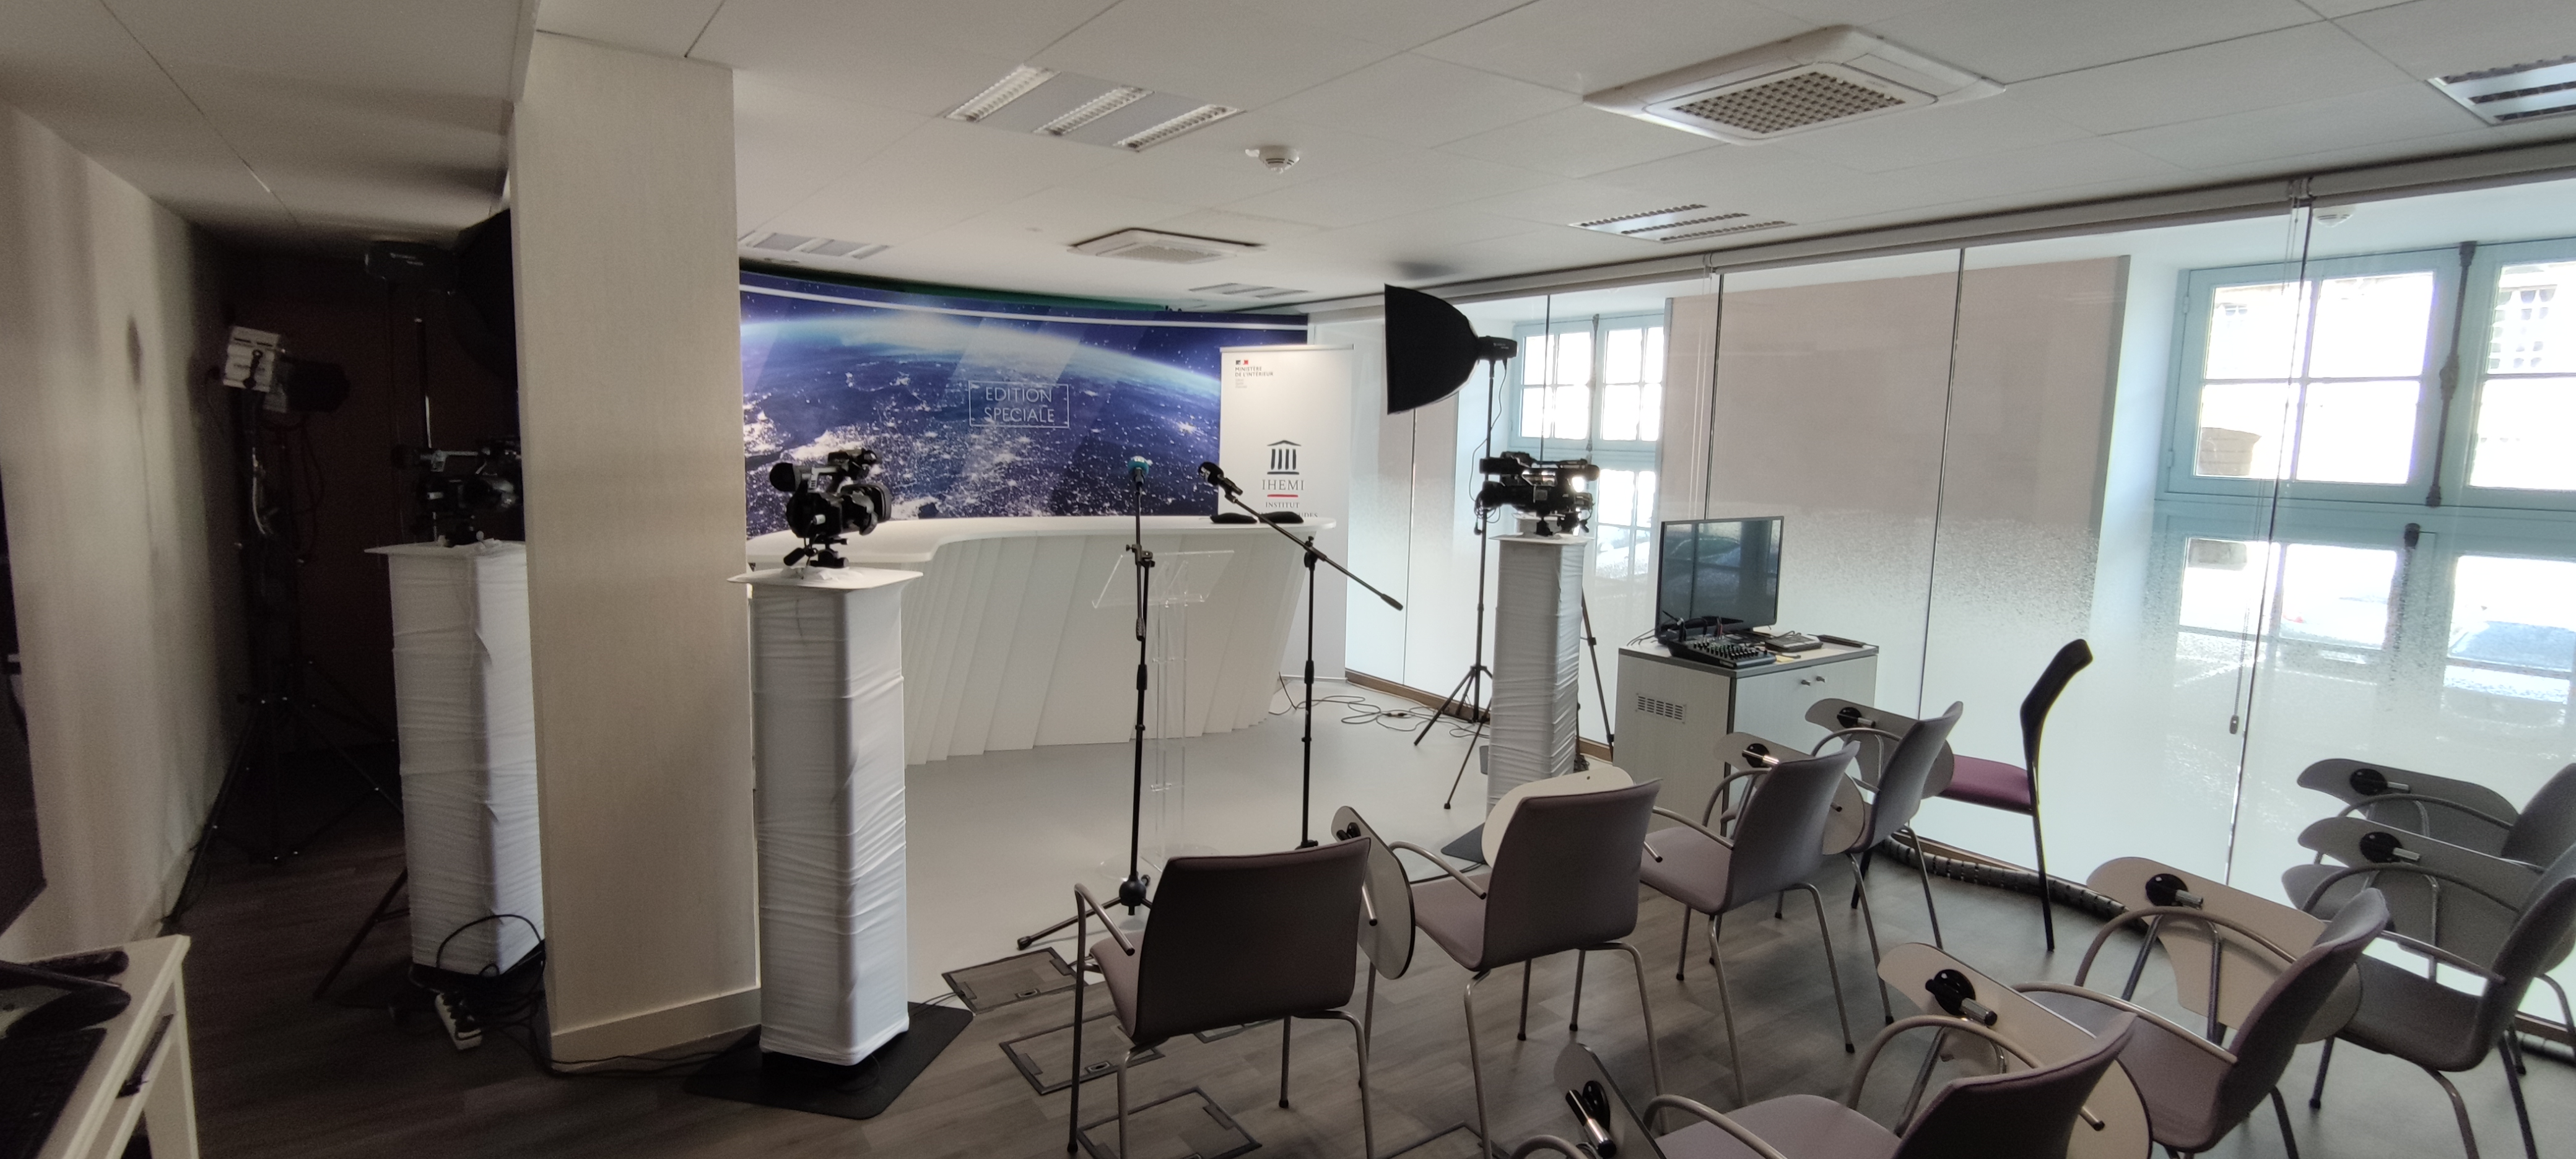
\includegraphics[width=0.95\textwidth]{figures/mediatraining.jpg}
    \caption{La principale salle de media training ; source : personnel}
    \label{fig2}
\end{figure}

Dans cette salle sont organisés des exercices de communication de crise au cours desquels l’auditeur est mis en situation face à un ou des journalistes dont le rôle est joué par la chargée de communication ou des intervenants extérieurs. Cet exercice est mis en place à la suite d’un cours de communication de crise. J’ai, au cours de mon stage, pu assister à trois types d’exercices : une communication auprès des médias, rapide et suivie d’un jeu de questions-réponses avec les journalistes ; le même format en extérieur sous forme de « micro tendu », et enfin un débat entre deux auditeurs sur un sujet préparé à l’avance, animé par un membre de l’équipe. Ces exercices se font à l’extérieur ou dans l’une des salles de mediatraining (voir figure ~\ref{fig2})

Le plus souvent, l’exercice de communication de crise suit un exercice de mise en situation en gestion de crises, qui a lieu sur le second ensemble du plateau technique. 

Ce dernier se compose de deux salles : une salle de crise (voir figure ~\ref{fig3}), composée de postes informatiques et de tableaux tactiles. Les auditeurs sont placés en immersion : ils reçoivent des informations par courriel et par téléphone selon un scénario de crise fictif établi à l’avance et doivent comprendre la situation à laquelle ils font face puis prendre les décisions adéquates. Pour recevoir les informations et communiquer leurs décisions, ils peuvent contacter ou être contactés par un ensemble d’acteurs de la gestion de crise, dont le rôle est joué par l’équipe du DRC ou bien par des intervenants extérieurs. Depuis cette salle, toutes les actions des auditeurs peuvent être surveillées par les formateurs situés dans une salle adjacente. Une autre salle plus classique d’une capacité de huit personnes est également à disposition des auditeurs.
% figure ~\ref{fig3}
\begin{figure}[!t]
    \centering
    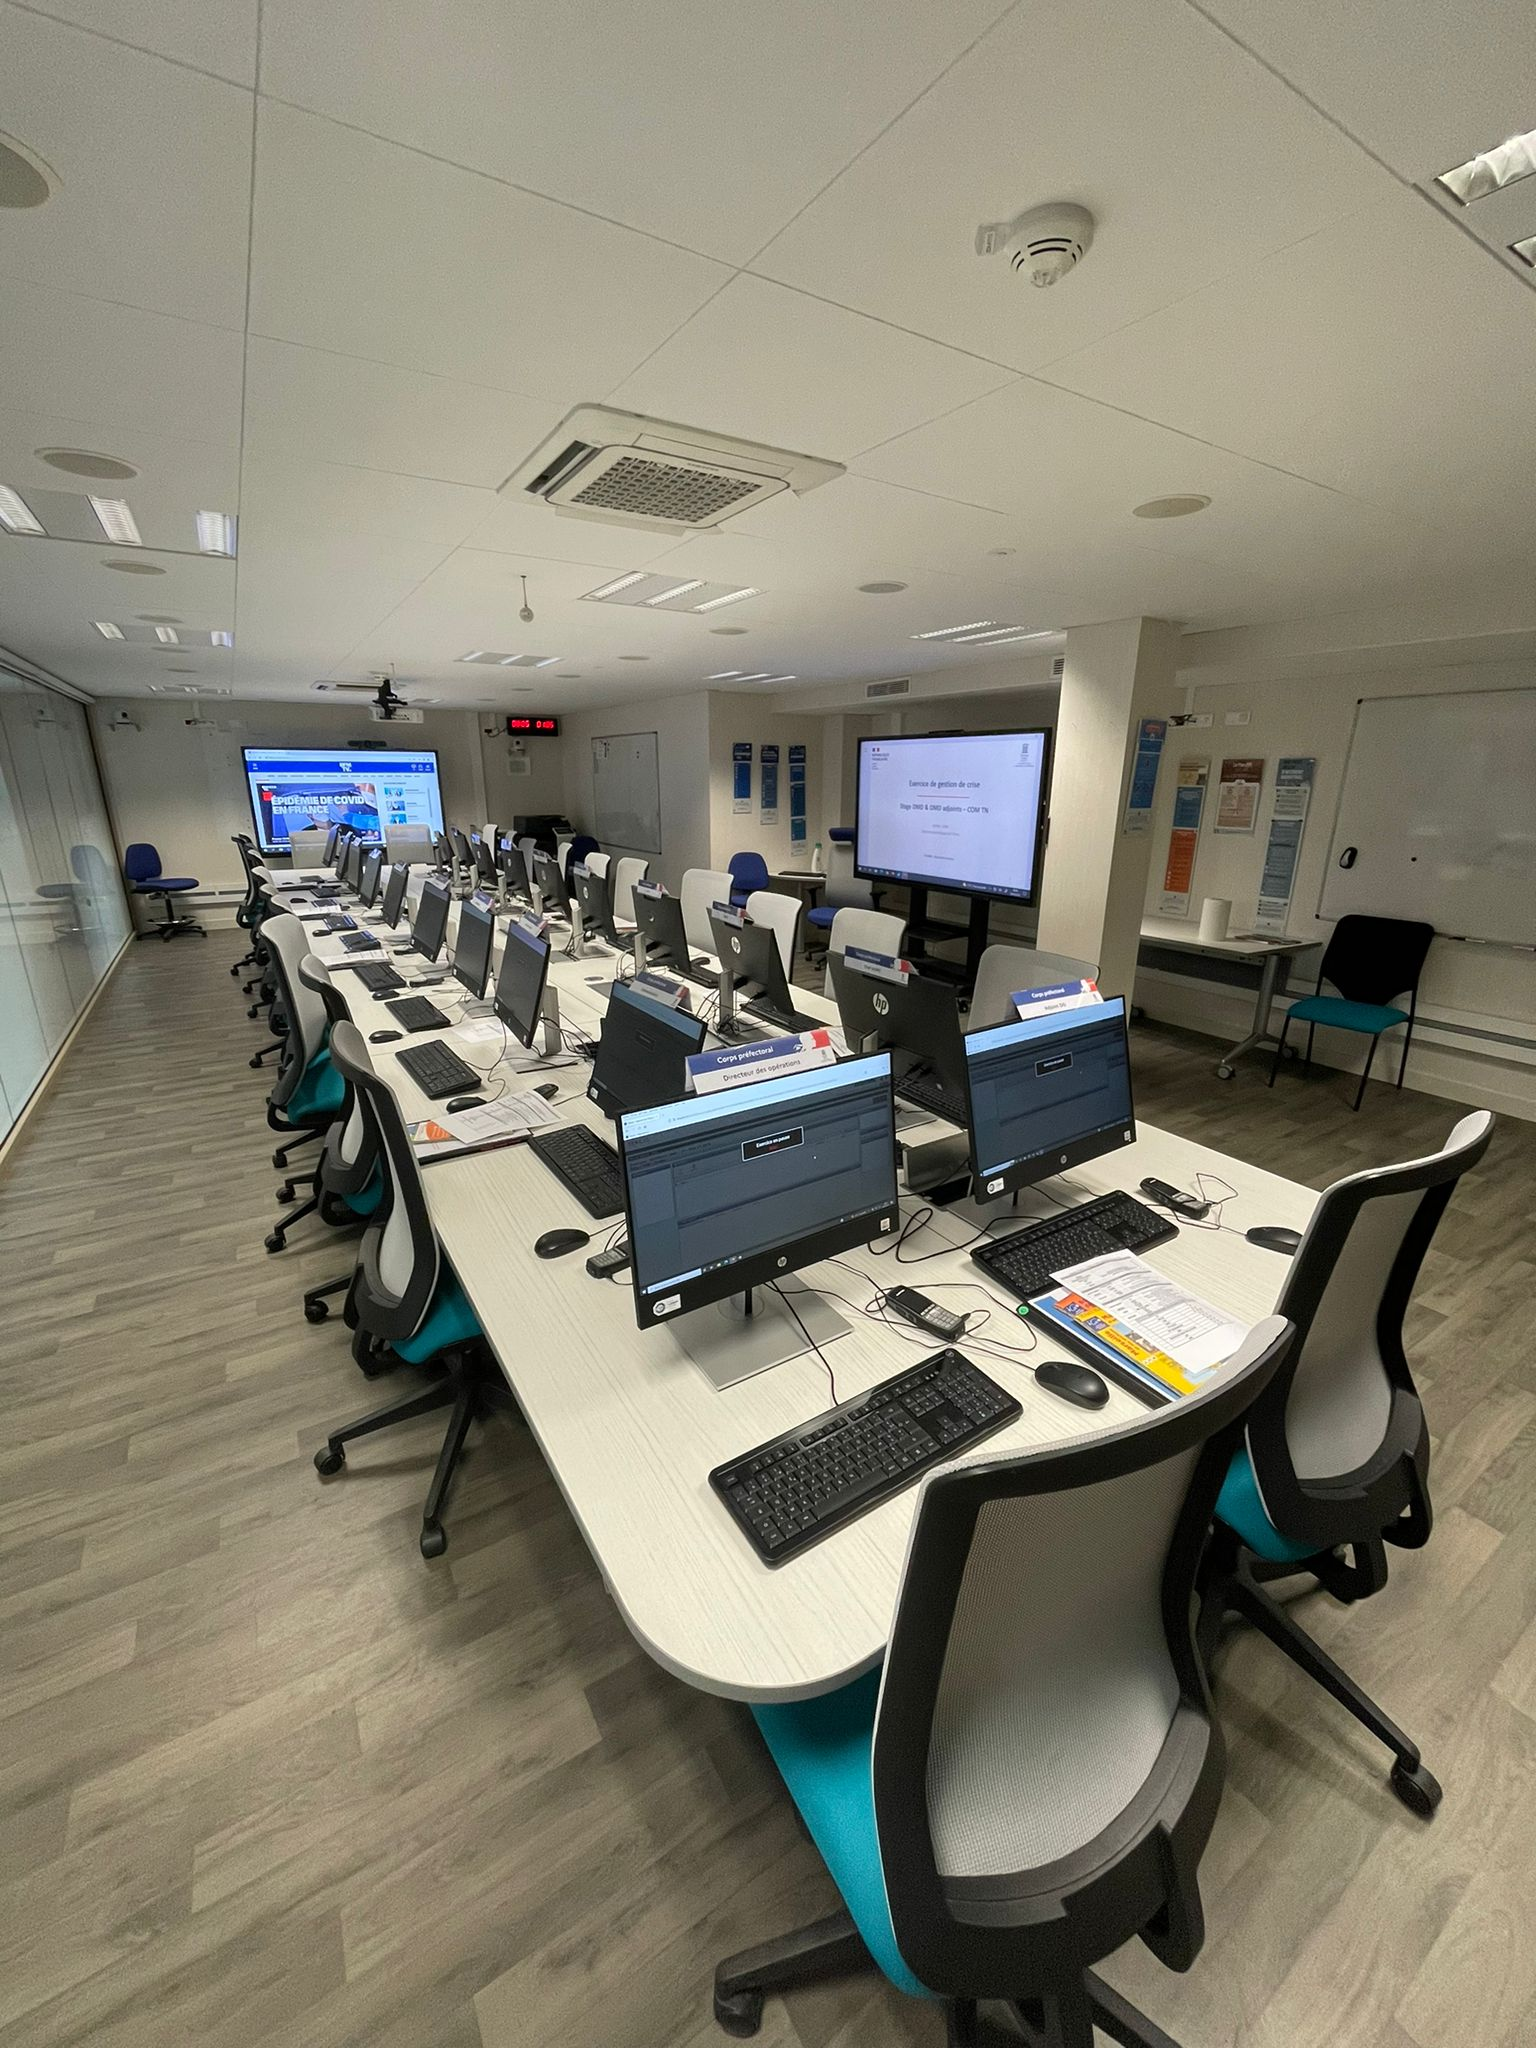
\includegraphics[width=0.7\textwidth]{figures/salledecrise.jpg}
    \caption{Salle de crise pédagogique du Département Risques et crises, source : personnel}
    \label{fig3}
\end{figure}

La présentation de ce plateau technique a deux objectifs. Elle montre d’abord la spécificité des moyens données au DRC. Les autres départements dispensent en effet la totalité de leurs cours sous forme de cours magistraux ou d’études de cas en salle classique. La majorité des formations dispensées par le DRC prennent aussi cette forme. Mais le déroulement de ces exercices pratiques et/ou immersifs est inédit par son caractère à la fois opérationnel pratique et le public de hauts dirigeants / hauts fonctionnaires ciblés. 

Rappelons donc rapidement les spécificités du DRC au sein de l’IHEMI : des formations portées par et à destinations d’internes à d’autres services d’autres ministères mais aussi une volonté d’affirmer une position externe à destination de tous les potentiels acteurs de la gestion de crise. L’IHEMI défend donc une image de référent à la fois dans la sphère institutionnelle et dans la sphère administrative. Tout en les reprenant, le DRC possède comme spécificité sa dimension opérationnelle avec des formations axées sur la pratique. Notons par ailleurs que j’y étais le seul cartographe, ainsi que le seul cartographe de l’IHEMI.

Cette sous-partie se veut également une introduction à l’environnement dans lequel j’ai été amené à répondre à un besoin en cartographie. En effet, l’équipe du DRC établit les scénarios des exercices de crise. La cartographie vient en appui à ces scenarios. 

Afin de détailler en quoi la réalisation de cartes s’intègre dans la création et l’utilisation de scénario à la gestion de crise, il convient de détailler ce que recouvre la gestion de crises. Ces deux points font en partie l’objet de la seconde partie de ce rapport.


\end{part}

\newpage
\thispagestyle{empty}
\mbox{}
\newpage

%%---------------------------------SECONDE PARTIE--------------------------------------

\begin{part}{La réalisation de cartes pour la formation à la gestion de crise : contexte, spécificités et types de cartes}

Cette seconde partie a pour objectif de montrer en quoi et de quelle manière la réalisation de cartes peut s’inscrire dans le contexte de la gestion de crises et particulièrement dans la formation à la gestion de crises.  Avant de nous intéresser au besoin en cartes du DRC pour ses formations et aux résultats, il convient de présenter ce que recouvre concrètement la gestion de crises. 

\mychapter{1}{Les caractéristiques de la gestion de crise}

\section{Qu’est-ce qu’une crise ?}

Tentons de donner une définition de ce qu’est une crise. Cette partie est essentielle pour comprendre l’origine du besoin en cartes dans une salle de crise, à fortiori sur le plateau technique pédagogique.
Les citations du paragraphe qui suit sont issue de l'article de \cite{borrazolivierQuEstceQu2020} pour CSO-Sciences Po.
Une crise se définit comme un « moment de rupture imprévisible et spectaculaire ». Dans le cas d’un état établi et sain qui se déroule de manière linéaire dans le temps, « la crise constitue une dégradation soudaine » (Cette définition est donnée dans le contexte de la médecine). Ce moment est central dans la situation de crise. Il a plusieurs implications. La première conséquence est la perte de sens : « tous les repères se dérobent et le monde ne fait plus sens » \parencite{lagadecGESTIONCRISES}. Ainsi, les situations de crise « présentent toujours un caractère imprévisible, surprenant, inédit ».  Cela implique également un « effacement des frontières organisationnelles » (CSO Sciences PO, 2020). Vu le caractère d’une situation de crise, le modèle institutionnel présente au mieux des limites et est, au pire, totalement inadapté à la situation. Voulant retrouver une situation connue, gérable et maitrisable, voulant sortir d’un après « trou noir » (Lagadec), il revient alors au décideur de réaliser un « cadrage politique » (CSO Sciences-Po, 2020). C’est-à-dire, face à cette absence de repères notamment institutionnels, coordonner les acteurs sur lesquels il a autorité. Face à une situation de crise, les objectifs sont donc multiples et s’enchaînent comme ceci. Compte-tenu la définition même de la crise, il s’agit de caractériser la situation de crise ou pour le dire autrement, répondre à la question à quoi faisons-nous face ? Ensuite, face à une organisation institutionnelle brouillée, place à la coordination des acteurs. Mais pour quel objectif ? Il s’agit face à la situation de crise donnée de garder opérants un certain nombre de services au détriment d’autres jugés moins essentiels. Les phases de caractérisation et de décision sont donc essentielles. 

Quid de l’anticipation pré-crise ? Des précisions me semblent ici nécessaires. Si une situation pouvant être problématique et/ou déstabilisante est suffisamment prévue, elle est de fait gérée sans accrocs et la crise n’est alors qu’un incident dont la solution est prévue. Prévoir un plan, une procédure pour quelque chose de prévisible évite de fait la crise. C’est donc une planification. Anticiper des écarts à une situation nominale théorique restreint de fait ceux-ci au domaine de l’incident. La crise n’intervient que lorsque qu’une conjonction de faits ou d’événements, souvent par leur enchaînement, échappent au(x) plan(s). Les accidents graves dans le secteur aéronautique en sont un exemple connu. 

Une anticipation que je décrirai « en temps réel » peut aussi être conduite en surveillant les signaux faibles. Un second type d’anticipation est en fait communément admis : il s’agit de l’anticipation durant la gestion même de la crise. Il est aussi intéressant d’anticiper les événements qui pourraient se produire, s’enchaîner, y compris au sein même de l’organe de gestion de crise (en pratique, la salle de crise, qu’il convient d’isoler de la crise elle-même \parencite{lagadecGESTIONCRISES}). Anticiper également les conséquences des décisions, qui pourraient empirer la situation, prises dans l’incertitude. Il s’agit alors d’ « éviter d’ajouter de la crise à la crise » \footnote{Anne-Lise Cœur-Bizot, 2022}. Le dernier moment de la crise est le retour à une situation nominale. La capacité à retrouver cette situation nominale, stable, connue, maîtrisée, après une crise par définition chaotique est appelée résilience. Il convient alors, pour améliorer la résilience, de réaliser un retour d’expérience (appelé RETEX ou REX selon les structures), qui participe à améliorer la préparation et la planification.

Précisons enfin qu’à la gestion de crises est associée la communication de crise réalisée pour limiter l’impact de la crise sur la population, ce qui passe souvent par la communication des décisions prises. C’est aussi assurer un positionnement pour le décideur / l’autorité : assurer une position de référence et de transparence face à un contexte d’inquiétude, de doutes sur les situations et sur l’autorité. Mais aussi dans un contexte de circulations de fake news, comme dans l’exemple de Lubrizol, où la majorité des tweets relayaient en réalité de fausses informations. \parencite{a12h31IncendieUsineLubrizol2019}

Pour terminer, nous avons entrevu qu’une crise se présentait sous un phénomène cyclique. La figure (voir figure ~\ref{fig4}) ci-dessous récapitule ces phases : pré-crise ou phase préliminaire avec veille prévention et planification, et le redressement, moment de rupture, période de chaos, retour à la normale. La communication s’y inscrit pleinement dans un schéma semblable (voir figure ~\ref{fig5})
%figure ~\ref{fig4}
\begin{figure}[!t]
    \centering
    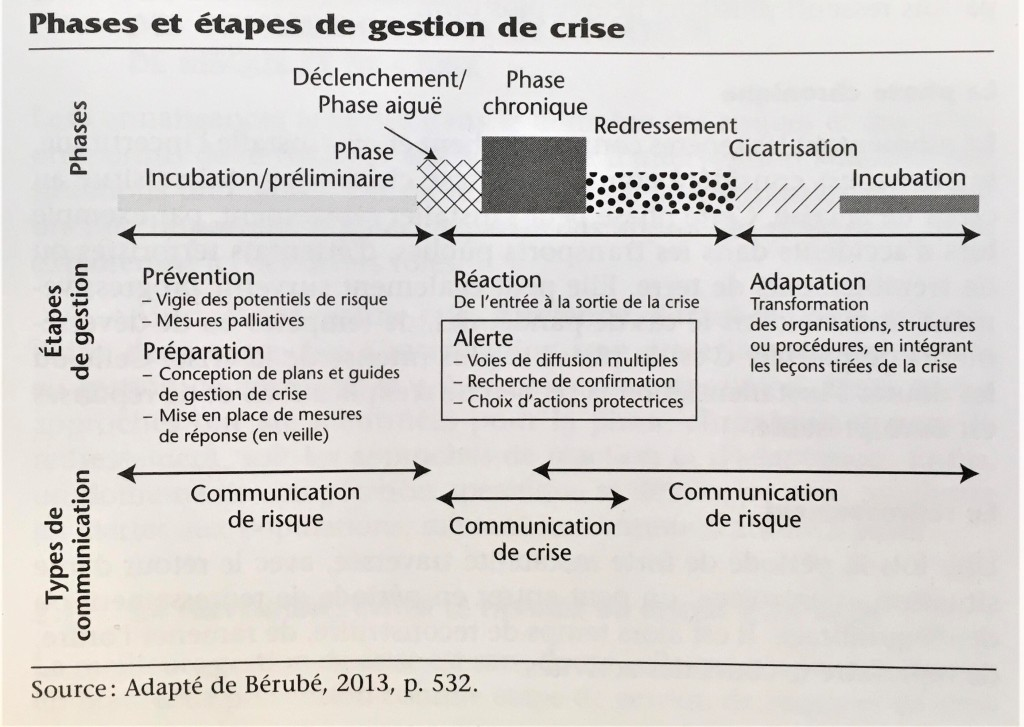
\includegraphics[width=0.95\textwidth]{figures/phasescrise.jpg}
    \caption{présentation des phases de la crise, source : OMSRP}
    \label{fig4}
\end{figure}

%figure ~\ref{fig5}
\begin{figure}[!t]
    \centering
    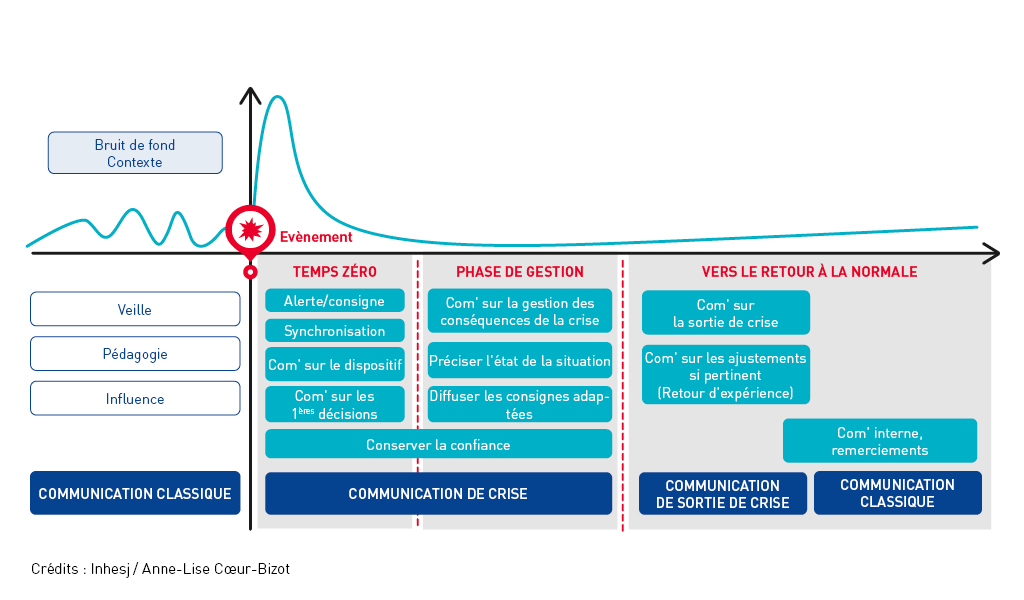
\includegraphics[width=0.95\textwidth]{figures/tempszero_crise.jpg}
    \caption{Les phases de la communication de crise, source : Anne-Lise Coeur-Bizot, INHESJ}
    \label{fig5}
\end{figure}

A ce stade, l’utilité de la réalisation de cartes apparaît déjà en réalité à chaque étape d’une crise et de sa gestion. 

Lors de la planification tout d’abord. Il s’agira alors d’identifier des vulnérabilités potentielles et leur impact : il s’agit alors de spatialiser les risques. Peuvent y figurer les mesures prévues par un plan. Les sapeurs-pompiers élaborent par exemples des cartes dites DFCI pour anticiper la lutte contre les feux de forêt sur lesquelles figurent les installations prévues à cet effet (bouches, citernes, lacs, chemins etc.)

Lors de la gestion de la crise, après son déclenchement, lors de l’anticipation des décisions prises en salle de crise, une analyse sur logiciel SIG permet par exemple d’estimer l’impact d’une décision. On pensera par exemple au nombre de personnes à évacuer dans un périmètre donné. Mais surtout, lors du moment de rupture, de déclenchement, et dans la phase de qualification de la crise qui suit. A ce titre, une simple carte de localisation peut suffire. A la question centrale qu’est-ce qu’il se passe ? une carte de localisation permet de répondre également à la question où cela se passe-t-il ? L’utilisation de l’outil cartographique est donc pleinement justifiée durant une crise. Il joue un double rôle d’aide à la compréhension et d’aide à la décision. Et la dimension spatiale n’est pas superflue. Le chapitre suivant présente les acteurs engagés dans la gestion de crise en France. Il permet de comprendre ensuite le fonctionnement de la salle de crise pédagogique de l’IHEMI et comment mes missions de réalisation de cartes s’y intègrent. Mais nous rappellerons que, compte tenu en France de la décentralisation et de la déconcentration, si le panel d’acteurs engagés dans la gestion de crise dépend de l’intensité de celle-ci, il dépend aussi de son emplacement géographique et de tout un jeu de compétences territoriales entre les acteurs publics.

\section{Les acteurs institutionnels incontournables de la gestion de crises en France}

Ce sous-chapitre a pour objectif de présenter comment sont gérées les crises en France, en mettant l’accent sur l’échelon départemental. C’est cet échelon qui est mis en avant à l’IHEMI. Le plateau technique du DRC et sa salle de crise reproduisent en effet une salle de crise de préfecture de département. C’est aussi le préfet, en tant que représentant de l’État et de son autorité dans son département, qui apparaît comme le principal décideur lors d’une crise importante. C’est à cet échelon que la stratégie de gestion d’une crise est établie : le préfet est « directeur des opérations » selon la directive ORSEC (hors crise exceptionnelle majeure, gérée au niveau national).

\subsubsection{La rencontre de plusieurs corps de métier}

L’organisation des différents services de l’État, « en cas de catastrophe », est prévu par le dispositif ORSEC (« Organisation de la Réponse de Sécurité Civile ») \parencite{ministeredelinterieurDispositifORSEC}, sous l’autorité du préfet. Ce dispositif, ainsi que le suivi national de la gestion de la crise par le niveau départemental, sont réalisés par la DGSCGC, direction du ministère de l’Intérieur. Le plan ORSEC permet de réunir des moyens issus de différents corps de métier au sein d’une disposition spécifique  : le Centre Opérationnel Départemental (COD), et ce alors que chacun travaille habituellement avec ses propres méthodes, avec une grande autonomie relative.

Il s’agit de coordonner les acteurs suivants

\begin{itemize}
    \item Ordre public
    \begin{itemize}
        \item Police Nationale. Les différentes directions de la police peuvent être mobilisées. DDSP pour la sécurité publique, PJ pour le volet enquête judiciaire, RAID ou BRI pour l’aspect intervention, PAF en cas de crise à dimension transfrontalière par exemple.
        \item Gendarmerie : là aussi, les gendarmes ont leurs propres services de sécurité publique, de maintien de l’ordre, d’intervention, d’enquête, de PTS etc.
    \end{itemize}
    \item Sécurité civile
    \begin{itemize}
        \item Sapeurs-pompiers, normalement rattachés à un état-major départemental au sein d’un SDIS.
        \item Autres moyens : on regroupe dans cette catégorie les associations agrées de sécurité civile, souvent mobilisées en amont sur des évènements et pouvant être appelées en renfort.
    \end{itemize}
    \item Armées :
    \begin{itemize}
        \item[] Délégué militaire départemental. Les militaires disposent d’importants moyens logistiques pouvant être utilisées lorsque les moyens civils sont indisponibles ou insuffisants
    \end{itemize}
    \item Les magistrats, bien qu’ils interviennent plus tard, dans un second temps qui est le temps de l’enquête
    \item Les élus. On pensera par exemple aux maires, au plus proche du territoire touché par exemple, en en charge du Plan Communal de Sauvegarde (PCS) et ayant le statut d’OPJ.
    \item Services déconcentrés spécialisés de l’État au niveau départemental, dans différents domaines : DDT, ARS par exemple
\end{itemize}

\subsubsection{Une structure hiérarchique et territorialisée.}

Lister les acteurs pour montrer leur variété ne suffit pas. Il convient de préciser que le dialogue et la « rencontre » entre ces acteurs se fait aussi de manière verticale. Pour un même acteur public, chaque échelon territorial (local, départemental, régional (ou « zonal »), national) dispose de compétences clairement définies. Ainsi, en cellule de crise, l’ARS doit par exemple dialoguer avec le CORRUSS (le centre de crise de ministère de la Santé, au niveau national) ou avec les directions de centres hospitaliers (niveau local). Cette imbrication est montrée par la figure ~\ref{fig6}. . Concernant la gestion de crise en elle-même, sous la direction du préfet, les compétences de chacun sont aussi clairement définies. La gestion opérationnelle-tactique de la crise par exemple, est réalisée au sein d’un PCO avancé, sur le lieu de la crise. Le préfet / directeur des opérations, doit être isolé de la crise, dans une salle de crise dédiée en préfecture. Il assure donc le lien entre le niveau tactique sur site et rend compte à l’État dans son échelon zonal et national, qui peut prendre le relais pour certains aspects au besoin et dans un second temps, selon concertations. 
%figure ~\ref{fig6}
\begin{figure}[!t]
    \centering
    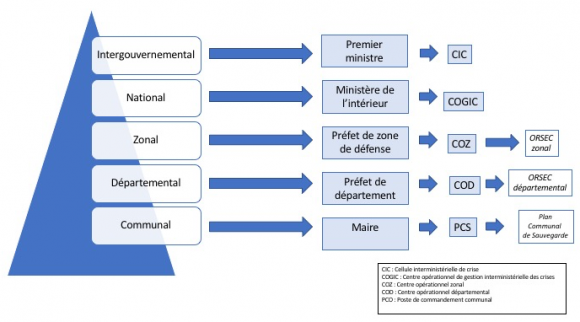
\includegraphics[width=0.95\textwidth]{figures/acteurs_crise.png}
    \caption{: les acteurs de la gestion de crise et leur niveau territorial ; source : Reghezza-Zitt, Jon (2018)}
    \label{fig6}
\end{figure}
Rappelons également que, pour un même acteur existe un enchevêtrement de compétences et de spécificité territoriales complexes. Lors de la réalisation de cartes dans la salle de crise pédagogique de l’IHEMI, il m’était par exemple régulièrement demandé si une zone d’intérêt se trouvait en zone Police ou en zone Gendarmerie, déterminant donc quel acteur avait compétence pour une intervention de type sécurité publique. (Je disposais, à ce moment, de la couche de données géographiques appropriée à cette question. Mais l’accès et la nature de la donnée est une question importante que nous évoquerons plus loin…). Concernant les spécificités fonctionnelles d’un même acteur, nous pourrons par exemple citer le cas des sapeurs-pompiers. 

Ces derniers sont des fonctionnaires territoriaux, rattachés à l’échelon département. Leur État-Major est un SDIS. Exception faite à Paris où les sapeurs-pompiers sont rattachés à l’armée de terre (BSPP) et à Marseille, où ce sont des marins (BMPM). De la même manière, en plus du découpage police-gendarmerie, en Ile de France, la police est gérée à Paris et en proche couronne par une structure dédiée : la Préfecture de Police (PP). Des statuts et formes différents pour des organisations internes différentes.

L’organisation en elle-même de la coordination des acteurs de la gestion des crises revêt une dimension territoriale complexe et pourrait à elle seule faire l’objet d’analyses territoriales et de besoin en cartes complexes. De plus, chaque acteur dispose souvent pour lui-même d’informations géographiques ou de supports cartographiques métier avec une culture et des pratiques propres. A ce titre, les sapeurs-pompiers et les militaires ont par exemple une pratique cartographique spécifique, des produits finaux et même une symbologie spécifique.

\mychapter{2}{Le plateau de crise de l’IHEMI : un Centre Opérationnel Départemental à vocation pédagogique}

\subsubsection{Déroulement d’un exercice de crise}

La salle de crise pédagogique du plateau technique du Département Risques et Crises que j’ai présenté dans la partie I B. 3 peut être configurée pour reproduire plusieurs dispositifs institutionnels. Pour quasiment chaque exercice de crise pour lequel j’ai été mobilisé – et il s’agit de sa configuration par défaut - la salle était préparée pour reproduire un Centre Opérationnel Départemental (COD). Plus précisément, et faisant écho aux acteurs et principes présentés précédemment, le site du ministère de l’Intérieur présente le COD tel que suit : 

% citation, minInt
Le COD est un outil de gestion de crise à disposition du préfet qui l'active quand un événement majeur a lieu dans son département (importantes manifestations, épisode climatique impactant la sécurité routière, accident de grande ampleur...). Présidé par le préfet, il rassemble l'ensemble des acteurs de la sécurité civile, la police et la gendarmerie nationales, les services de l'Etat concernés et les représentants des collectivités. \parencite{ministeredelinterieurQuEstceQu}

Dans la salle de crise pédagogique de l’IHEMI en configuration COD, les acteurs typiques d’un COD tel que spécifié par le dispositif ORSEC, sont disposés tel que visible sur la figure ~\ref{fig7}. Chaque acteur gère les aspects de la crise qui entrent dans son champ de compétences. Notons que les effectifs du SIDPC, service présent en temps normal en préfecture, ont en charge la coordination et la synthèse dans la salle de crise. A ce titre, ils tiennent à jour une main courante des informations reçues et des décisions prises. Chaque action doit y être consignée. Chaque pôle dispose d’un poste informatique sur lequel est installé un logiciel spécifique à la mise en place d’un scénario de crise.
% figure ~\ref{fig7}
\begin{figure}[!t]
    \centering
    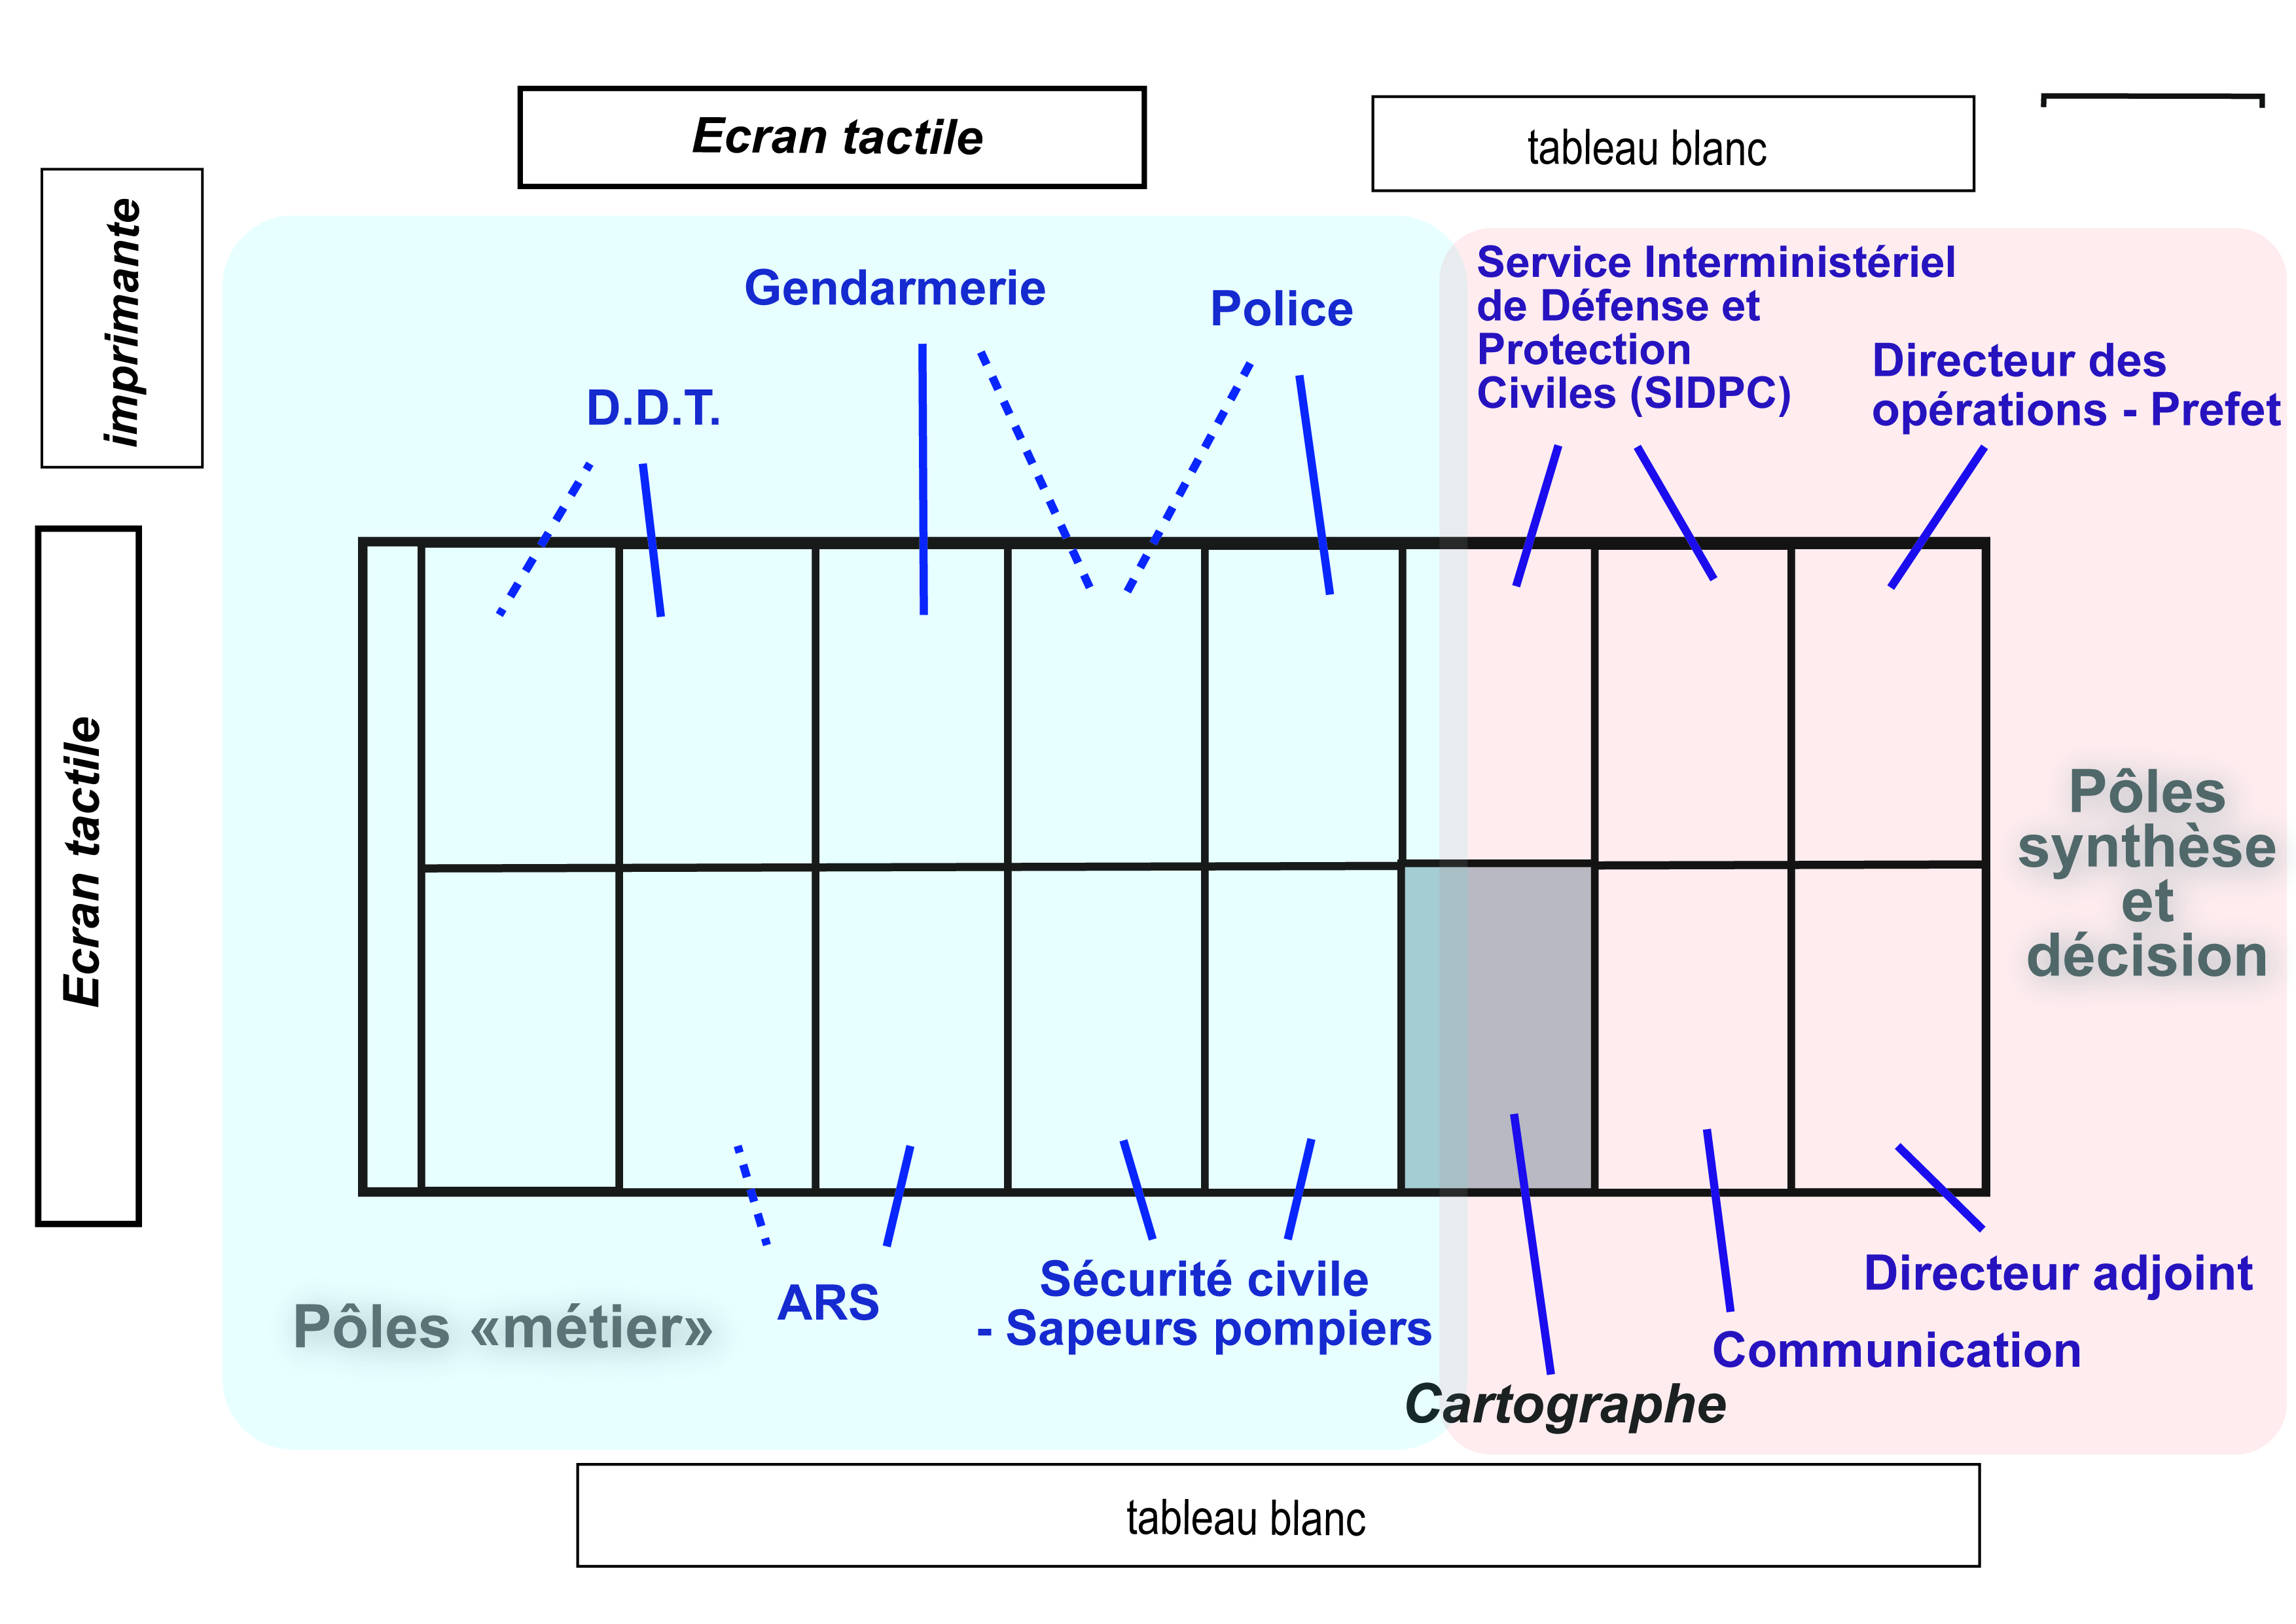
\includegraphics[width=0.95\textwidth]{figures/COD_plan.jpg}
    \caption{Organisation spatiale des rôles en salle de crise en configuration COD, source : personnel}
    \label{fig7}
\end{figure}

Précisons comment se déroule un exercice. Celui-ci dure une demi-journée. Après un cours théorique sur la dynamique et les éléments à prendre en compte en gestion de crise en COD, chaque auditeur choisit un rôle et se positionne au poste correspondant. Des évènements et informations qui sont établies à l’avance dans un scénario lui sont notifiés au moyen d’un téléphone ainsi que par courriel au travers du logiciel dédié (nommé Pixcis) installé sur les postes. Ces éléments sont cadrés dans un groupe horaire spécifique à chaque scénario. Ces notifications proviennent d’acteurs institutionnels autres, ou du même organisme mais à un échelon territorial inférieur ou supérieur, qui sont joués par les animateurs de l’exercice présents dans une salle dédiée située à côté de la salle de crise. Il y a donc une salle « joueur » et une salle « animateur ». Les joueurs doivent donc conjuguer avec des éléments et acteurs extérieurs. Ils sont également observés et surveillés par l’équipe animateurs. L’ensemble de l’exercice est encadré par un directeur d’exercice (DIREX), qui a notamment pour tâche d’adapter l’enchainement d’événements et d’informations envoyés aux joueurs. Ces éléments et informations sont appelés \textit{inputs}. Il a aussi pour tâche, supplée par un coordinateur, d’observer leurs réactions et décisions. Il coordonne aussi les autres animateurs. Chaque animateur, s’il joue un rôle, est en réalité un spécialiste métier : les rôles qu’il joue sont choisis en fonction de ses compétences. Par exemple, le rôle externe du CROGEND (Centre de renseignement opérationnel de la gendarmerie) est joué par un gendarme de l’équipe de l’IHEMI. Les joueurs, dans le rôle qu’ils jouent, sont donc confrontés à une situation de crise qu’ils doivent gérer. 

Dans une situation idéale, chaque pôle métier fait remonter les informations au pôle coordination-synthèse, qui les consigne dans la main courante. 

J’ai ensuite à charge, en coordination avec ce pôle, d’alimenter un support cartographique présentant les informations d’intérêt stratégique, avec les spécificités que cela implique : sélection, hiérarchisation et simplification de l’information. Et ce, pour que le décideur ait une vue synthétique et spatialisée de la situation en temps réel. D’autant plus que ce dernier n’a pas toujours une bonne connaissance du territoire sur lequel il a autorité. C’est donc, en situation dégradée, la fois une aide à la compréhension, une aide à la décision et outil de suivi des décisions.

\subsubsection{Demandes de cartes en situation de gestion de crise}

Dans ce cadre, je disposais, au sein de la salle de crise, d’un poste doté du logiciel QGIS et étais placé à disposition des joueurs. Je leur précisai, en début d’exercice lors du point sur les modalités de celui-ci, avec quel moyen je pouvais leur mettre des productions cartographiques. Plusieurs moyens étaient à ma disposition : montrer une carte directement sur mon poste à un des joueurs qui vient me solliciter, imprimer une carte, ou bien enfin la diffuser sur l’un des grands écrans tactiles de la salle. La figure ~\ref{fig8} présente un exemple du type de production cartographique, alimenté en temps réel, que j’ai pu produire. Détaillons quelques points de ce type de réalisation.
%figure ~\ref{fig8}
\begin{figure}[!t]
    \centering
    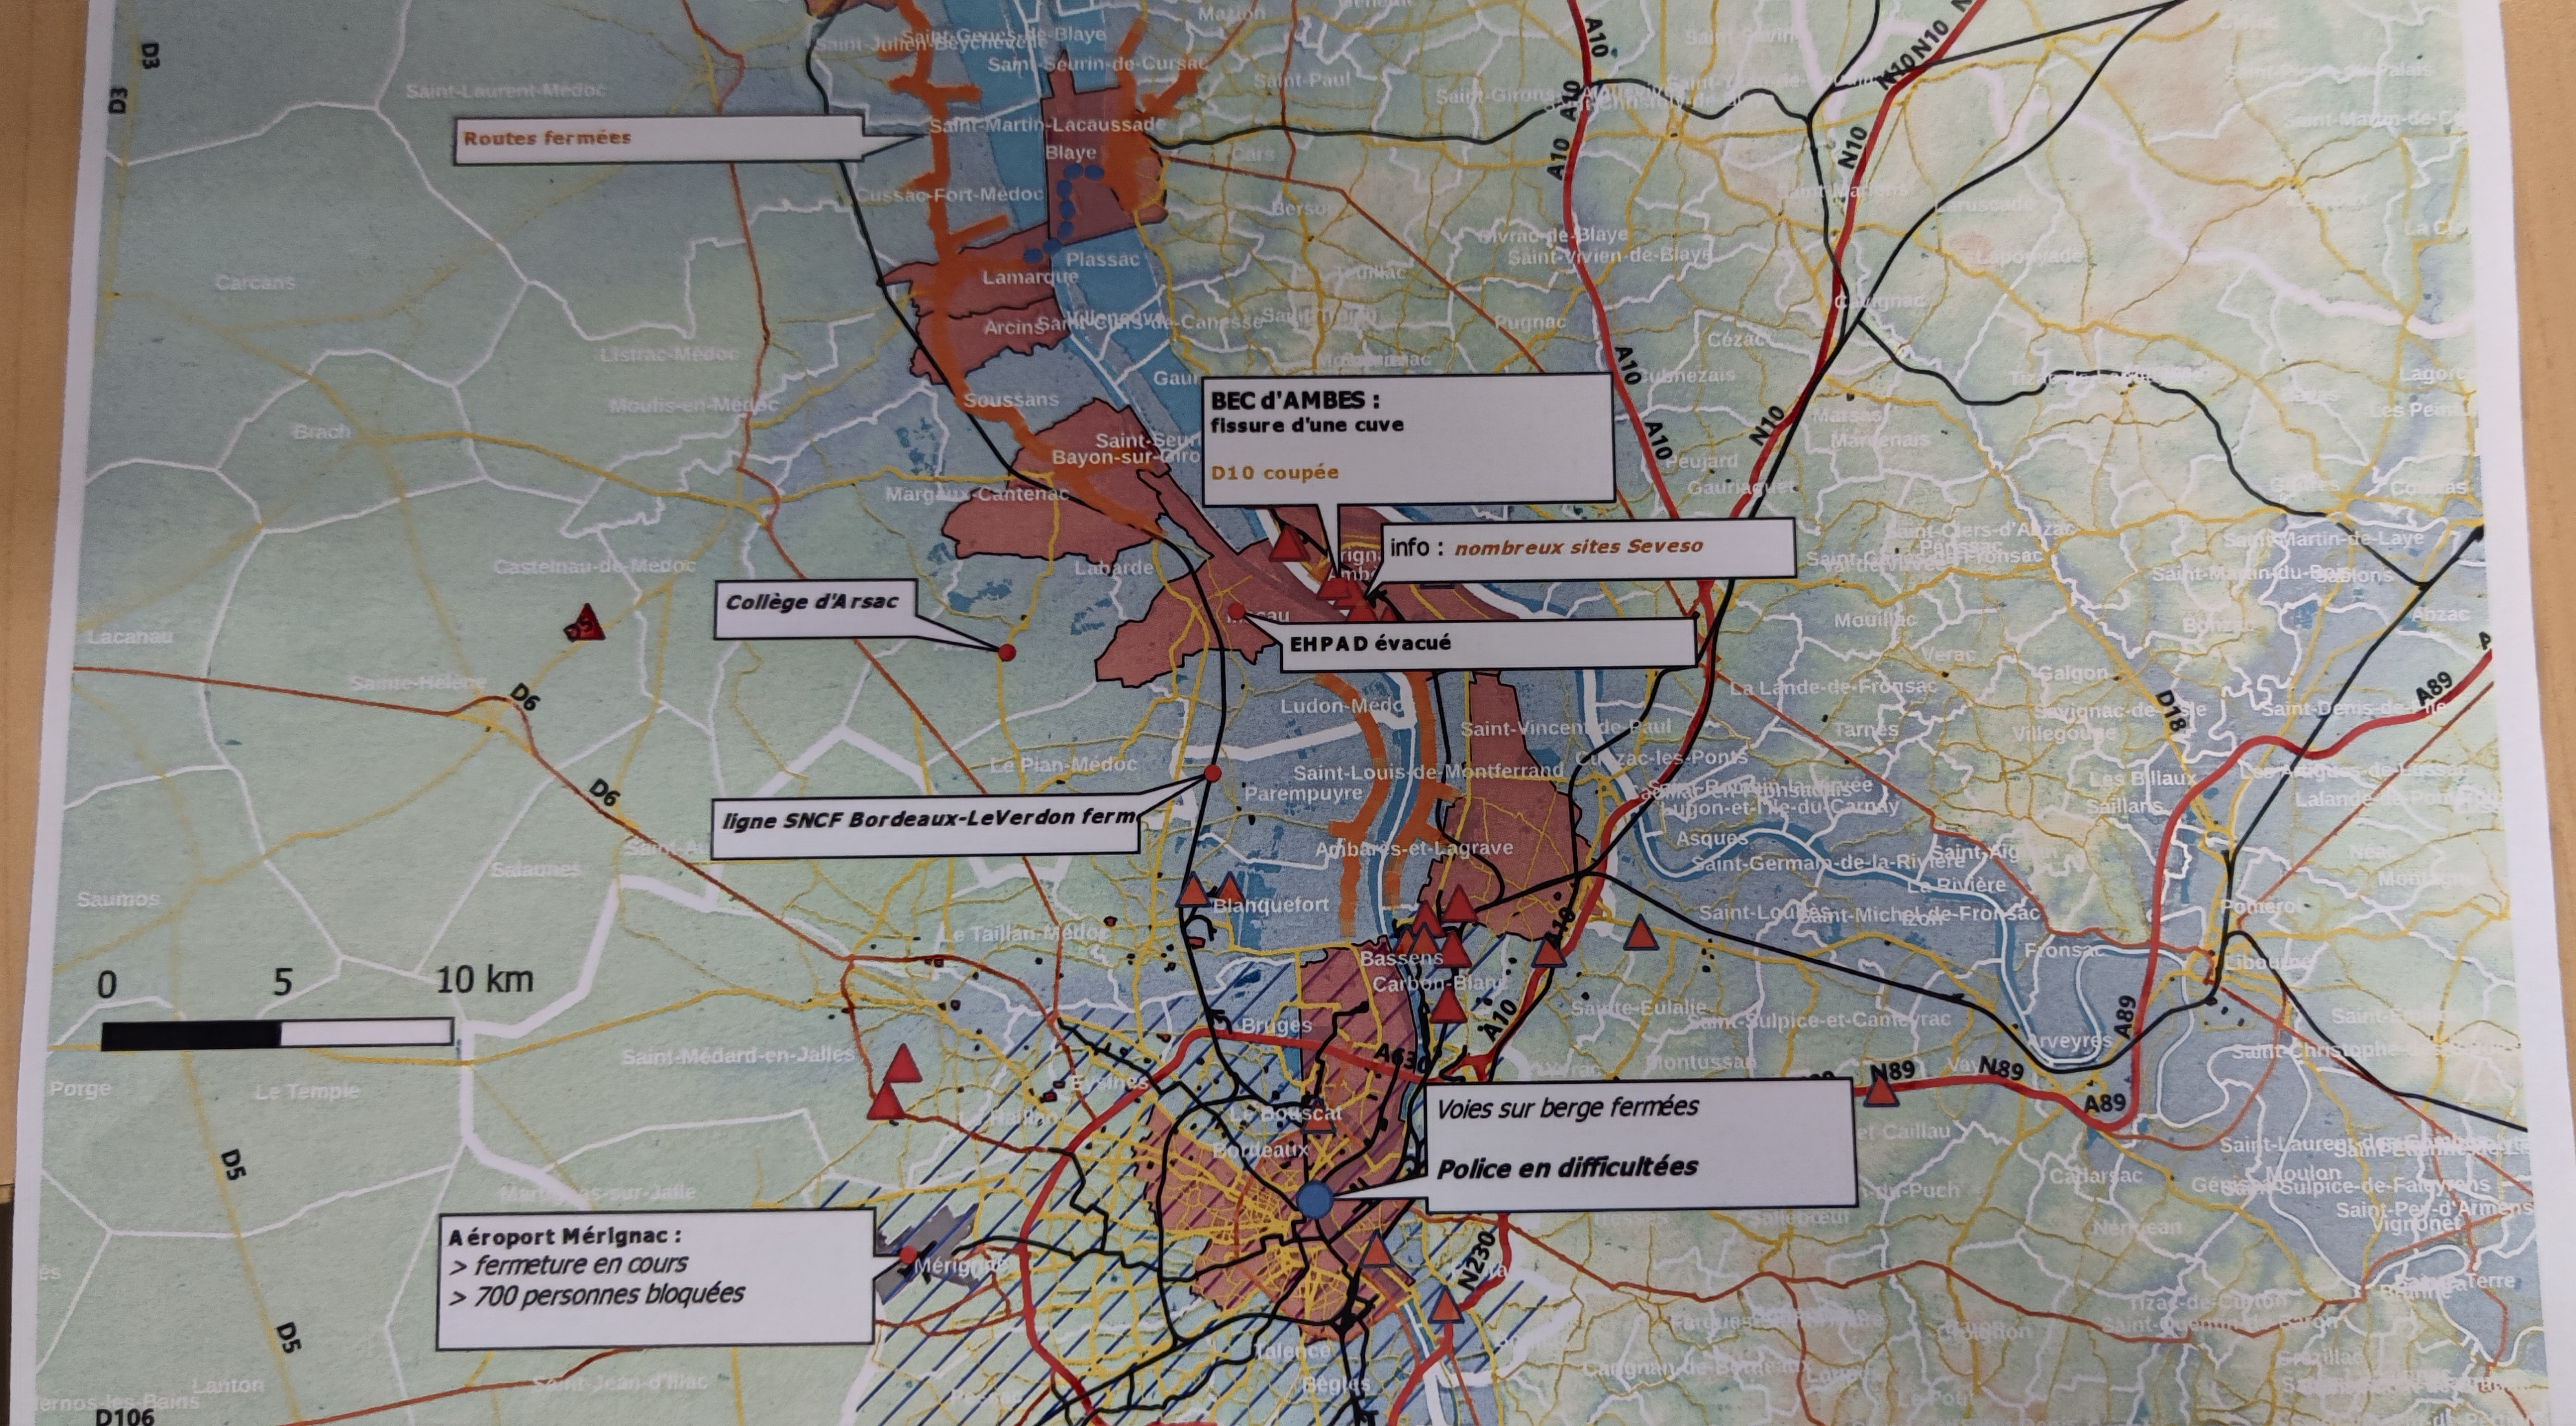
\includegraphics[width=0.95\textwidth]{figures/EOLE33_support.jpg}
    \caption{Exemple d’un support cartographique alimenté en temps réel en salle de crise, ici dans le cadre d’un scénario mettant en scène une inondation dans l’estuaire de la Gironde, source : personnel}
    \label{fig8}
\end{figure}

\paragraph{Préparation des données}
Connaissant à l’avance quel scénario de crise sera joué, je pouvais préparer un fond de carte avec des informations « prêtes à l’emploi » en fonction de ce que je jugeai pertinent à proposer aux joueurs. Après quelques exercices, et selon le profil des auditeurs-joueurs, il m’arrivait d’anticiper – avec un succès parfois relatif - quel type de données ces derniers me demanderaient. Dans l’exemple de la figure ~\ref{fig8}, le scénario joué met en scène une situation d’inondations et de tempête dans l’estuaire de la Gironde : la représentation du relief et de l’altitude est préparée en amont de l’exercice à l’aide d’un MNT. Mon fond de carte est proposé ensuite aux joueurs pour donner suite à une première expression d’une demande de leur part ou bien de mon propre chef en début d’exercice. Préparé en pleine connaissance du scénario, il n’est donc pas neutre . De plus la préparation des données était personnelle : l’IHEMI ne disposant pas de jeux de données géographiques métiers pour ses exercices, j’étais libre et autonome dans le choix de ceux-ci et dans la préparation en amont de mon environnement de cartographie en salle de crise durant les exercices.

\paragraph{Expression du besoin, circulation de l’information et positionnement professionnel et psychologique des joueurs.}
Les demandes concernant la cartographie n’étaient, lors des exercices, en rien formalisées ou complètes. Deux raisons à cela. Premièrement, les joueurs ne sont pas des cartographes, ni même des spécialistes du rôle qu’ils jouent dans le COD : il est ainsi parfois nécessaire de leur expliquer les possibilités de réalisation, des données dont je dispose. La disponibilité et la nature des données est par ailleurs un aspect totalement méconnu ou au mieux ignoré par ceux-ci. Lors d’une demande impossible à réaliser dans un délai raisonnable, naissait alors souvent de la frustration et de l’incompréhension dans l’esprit du joueur. D’autant plus lorsque le but de l’exercice est, de plus, en partie de les former à la circulation de l’information en contexte dégradé et chaotique de la crise que nous avons décrit plus haut. Et c’est, deuxièmement, cet aspect qui fait que, selon les situations et le profil des joueurs, leurs attendus et leur comportement diffèrent. Lors des debriefings des exercices, certains, peu enclins à dialoguer avec le pôle cartographie – ni avec d’autres acteurs d’ailleurs - ont par exemple exprimé qu’ils auraient souhaité avoir un cartographe force de proposition, venant les voir, là où j’avais pour consigne, dans un premier temps de l’exercice, de rester en retrait et de seulement répondre aux demandes des joueurs s’adressant directement à moi, oralement ou par mail. D’autres, à l’inverse, prennent dès le début de l’exercice des décisions et instaurent, notamment en tant que directeur des opérations, des pratiques et des demandes à chaque pôle. Je suis dans ce cas immédiatement sollicité. Et si j’ai parfois, pour les raisons déjà évoquées, besoin de négocier les modalités de livraisons cartographiques, je suis tout de suite, dans ce cas, inclus dans le processus décisionnel. Malgré cela, le processus de circulation de l’information n’a été – lors des exercices auquel j’ai participé – que rarement en accord avec la circulation théorique attendue que nous avons décrit plus haut. Conséquence : au lieu d’avoir pour collaborateurs principaux les joueurs jouant le rôle du SIDPC en coordination-synthèse, il m’est arrivé de voir chaque pôle métier – police, SP, ARS… – venir me solliciter indépendamment de tout filtrage, recoupage, remontée d’information. En clair, chacun utilisait mes compétences et le support que j’alimentais indépendamment, en « silo métier ». 

Dans ce cas, il m’était demandé de proposer, en deuxième partie d’exercice et si cette demande ne m’avait pas encore été faite ou si je ne l’avais pas réalisé de moi-même, un support cartographique projeté sur l’un des écrans et placé à vue de tous. Cet outil permet en effet de rendre la carte visible pour en priorité le décideur - directeur des opérations - mais aussi pour chaque pôle métier. L’objectif recherché est alors d’utiliser la carte comme outil permettant une conscience situationnelle \footcite{officequebecoisdelalanguefrancaiseGrandDictionnaireTerminologique} partagée. L’utilisation et les demandes de cartes se positionnaient donc de façon plus ou moins éloignée, selon le profil métier des auditeurs placés en joueurs, de cette utilisation idéale, où la carte est alimentée en temps réelle, par des informations synthétisées, vérifiées, vues par tous comme outil de compréhension et d’anticipation partagé.  Par exemple, lorsque les auditeurs étaient des officiers supérieurs de gendarmerie, les demandes de cartes et le processus de remontée d’information, s’ils n’étaient pas toujours totalement pertinents, étaient clairement cadrés, dès le départ, chacun se mettant très vite dans son rôle, sous les ordres du DO. Ce positionnement peut s’expliquer par la culture de l’opérationnel, de la lecture de cartes topographiques, d’élaboration tactiques et d’une chaîne hiérarchique établie et respectée. Ces différences de processus s’expliquent aussi par le facteur humain, avec une question centrale en gestion de crise : Quels sont les biais et réactions des acteurs dans une situation de rupture, de chaos, de dérobement qu’est la phase aigüe de la crise ? Ainsi, dans ce temps-ci, certaines personnes se rattachent à des acquis, parfois non-pertinents mais faisant office d’ancrage, quand d’autres manifestent une certaine forme de dissociation, et ne traitent tout simplement plus les informations, ou plutôt les problèmes à gérer qui leur arrivent.

Ainsi, pour deux exercices où est joué un même scénario, chaque support cartographique est unique, et dépend de tous ces facteurs, essentiellement humains mais aussi à des caractéristiques mêmes de la crise.

Enfin, il m’a été quelquefois demandé, dans le cadre d’un exercice, de produire, indépendamment du support projeté, des cartes destinées à l’extérieur de la salle de crise. Des cartes à communiquer aux autres acteurs ou bien encore des cartes à publier auprès de la population fictive via le pôle communication. Les cartes sont alors en fait envoyées aux animateurs de l’exercice. Une nouvelle spécificité ici : je me devais alors de faire attention aux informations figurant sur la carte. Certaines, lors d’une crise, ne doivent pas être portées à la connaissance des autres acteurs. Impensable, par exemple, de faire sortir une carte comme celle de la figure ~\ref{fig8}, sur laquelle, en plus de l’absence d’habillage, figure le nombre de personnes décédées dans chaque situation liée à la crise, sans aucun contrôle de l’autorité judiciaire \footnote{Dans la gestion d’une crise, ce n’est pas le préfet mais le procureur qui rend public auprès de la presse le nombre définitif de victimes. Il le fait, de plus, dans un second temps. Dans un premier temps, le préfet doit, soit ne pas communiquer de bilan victimaire, soit tout au plus, en concertation avec le procureur, ne donner qu’un ordre de grandeur.}.

Pour résumer, l’environnement direct de réalisation et d’alimentation du support cartographique est en réalité baigné dans les caractéristiques de la crise. Celle-ci entraîne des acteurs de différentes sphères et de profils différents à collaborer dans un contexte de frontières institutionnelles dissolues et de dialogue direct. Les demandes cartographiques sont donc parfois impertinentes, farfelues, irréalisables, dans une situation ici volontairement rendue instable avec un processus de dialogue et de transmission de l’information revêtant une part d’improvisations et de biais psychologiques, à fortiori lorsque les personnes prenant place en salle de crise y sont dans le but de se former à ces mêmes processus. La carte dépend aussi de son public : interne ou externe à la salle de crise.

\paragraph{Délais de réalisation et temporalités}
Une spécificité essentielle des productions cartographiques en salle de crise durant l’exercice est le délai de réalisation très court. Les modalités de l’exercice précisent que les joueurs doivent produire sur demande de la CIC \footnote{Armée par le ministère de l’Intérieur place Beauvau en cas de crise d’importance nationale et qui concerne, comme son nom l’indique, plusieurs ministères} (Cellule interministérielle de Crise ) jouée par l’équipe animation, un point de situation écrit à intervalle régulier, de l’ordre d’une ou deux heures.  Il m’est souvent demandé de noter l’heure à laquelle la carte a été produite, ainsi que l’heure de chaque évènement majeur, afin d’aider le décideur dans sa compréhension temporelle des évènements. L’indication du groupe horaire est une pratique très présente chez les sapeurs-pompiers et les acteurs de l’ordre public.  Très souvent, une impression ou une capture d’écran du support cartographique projeté m’est demandée, cette fois-ci avec une mise en page et un habillage présent bien que succinct et la suppression de certaines informations \footnote{Notons par ailleurs que ces suppressions, pour les cartes communiquées à l'extérieur, ne me sont parfois pas explicitement demandées, le DO oubliant parfois que les acteurs réunis ou qu’un cartographe détaché en COD peut ne pas être familier de ces questions…} . De plus, cette carte projetée n'a – hors de ces demandes - pas vocation à être publiée ni même à sortir de la salle de crise. Ceci explique l’absence totale d’habillage de la carte, d’autant plus que le support est dynamique dû à l’interface tactile de l’écran de la salle. Dans l’alimentation de celui-ci avec les informations qui me sont remontées – normalement par le SIDPC mais, comme nous avons vu, souvent par les pôles métiers – le délai de mise à jour est ici presque réduit à néant. La réalisation reste alors purement dans la visualisation proposée par QGIS sur laquelle je place quelques annotations. Néanmoins, la hiérarchisation des informations est primordiale : le décideur doit pouvoir y lire rapidement les éléments les plus urgents et/ou les plus importants sans être perturbé par un habillage pouvant être superflu. 

Ces différentes demandes de cartes reflètent en réalité une imbrication subtile de différentes temporalités liées à la hiérarchisation des informations, événements, décisions apparaissant durant la gestion d’une crise. 

\mychapter{3}{Spécificités cartographiques à propos de la dimension pédagogique}
Nous avons présenté le type de carte qu’il m’a été donné de réaliser au cours des exercices de crise au profit des auditeurs, sur le plateau de crise. Mais le fait que la salle de crise soit à vocation pédagogique implique d’autres besoins en cartographie, et donc, me concernant, d’autres missions. Je m’attache donc dans ce chapitre à les présenter – avec leurs spécificités - après une brève explication préalable.

Lors de la conduite d’un exercice de crise, les \textit{inputs}, en bref toutes les entrées externes à la salle de crise – sont définies et crées en amont dans un scénario de crise fictif. Ce dernier est créé par l’équipe du DRC. Chaque \textit{input} est détaillé : groupe horaire du contexte de l’exercice, acteur expéditeur, acteur destinataire et enfin la réaction des joueurs attendue. Le scénario est intégré sous format numérique dans le logiciel Pixcis. Lorsque l’exercice est joué, les animateurs déclenchent manuellement les \textit{inputs} dont l’expéditeur est un acteur joué par un animateur donné. 
\newline
\begin{itemize}
    \item Les « planches animateur »
\end{itemize}
Or, les animateurs sont pour la plupart des intervenants extérieurs, indépendants ou fonctionnaires d’autres directions ou autres ministères. Ils ne connaissent donc pas aussi bien les scénarios que l’équipe du DRC.

Par conséquent, est distribué en début d’exercice, à chaque animateur, un dossier présentant le scénario. Il contient une contextualisation, un récapitulatif des événements auxquels seront confrontés les joueurs, les acteurs institutionnels à jouer ou ceux mentionnés dans le scénario. Est également affichée en salle animateur une carte topographique IGN au 1/25e de la zone dans laquelle le scénario se déroule. Cet outil permet, durant l’exercice, aux animateurs - donc aux collaborateurs intentionnels extérieurs au COD si on se place du point de vue joueur – de répondre à des questionnements contextuels. Par exemple, le représentant de l’ARS en COD (poste tenu par un joueur en salle de crise durant l’exercice) pourra demander au CORRUSS du MDS (rôle tenu par un animateur intervenant détaché du MDS) le nombre de lits disponibles dans l’hôpital le plus proche de la région. Ayant ces chiffres à disposition dans un tableau et la carte IGN à proximité immédiate, il pourra répondre à la question. 

Mais cet outil ne participe pas à la compréhension et à la prise de connaissance globale du scénario par les animateurs. C’est pour cela qu’il m’a été demandé de produire, pour certains scénarios, une planche cartographique, au format A3, vouée à être plastifiée et distribuée à chaque animateur en début d’exercice. L’objectif de ce support est d’offrir à chaque animateur une vue synthétique du déroulement temporel et de la répartition spatiale des principaux éléments du scénario. Le DRC souhaite, à terme, disposer d’une planche pour chaque scénario. La figure ~\ref{fig9} montre l’une d’entre elles. Elle concerne le même scénario que la figure ~\ref{fig8} . Sur cette carte figurent plusieurs types d’éléments. 
Premièrement, des éléments de contextualisation et de présentation du territoire, tel que l’altitude ou bien les chemins de fers. Ces éléments n’interviennent pas directement dans le scénario.  Deuxièmement, apparaissent les acteurs et compétences territoriales, avec par exemple : hôpitaux, caserne de SP, commissariat de police, brigades et compagnies de gendarmerie départementale, limites de commune, d’EPCI, de département, zones Polices et Gendarmerie. Et dernièrement, les éléments relatifs au scénario en lui-même, à la situation fictive de la crise. Cela implique une sélection, catégorisation et hiérarchisation des \textit{inputs}. A ces trois types d’informations s’ajoute un point essentiel : la représentation d’une frise chronologique des événements. Pour bien comprendre et jouer correctement un scénario de crise complexe, les animateurs ont en effet besoin de cette information. Ayant à leur connaissance les événements de l’intégralité du scénario dans l’espace et dans le temps, ils disposent donc d’une vision omnisciente du scénario, avant d’animer l’exercice et de se plonger dans la temporalité de la gestion de crise telle que vécue par les joueurs. 
Ces cartes, pour être homogènes d’un scénario à l’autre, voient leur habillage élaboré à partir d’un \textit{template} sur Adobe Illustrator.

Par ailleurs, le DRC réalise aussi des exercices de formation à la gestion de crise sous forme d’ateliers au cours desquels les principaux \textit{inputs} sont présentés au fur et à mesure aux auditeurs sur un diaporama. Ceux-ci, sous forment d’une discussion et d’un débat avec les animateurs, développent ensuite les décisions qu’ils auraient pris en salle de crise en tant que DO. Lors de ces exercices, deux ou trois planches sont, à chaque point de situation, distribuées aux joueurs. Une planche comme celle de la figure ~\ref{fig9} est dans ce cas déclinée en une version comportant les informations passées, mais épurée des informations à venir pour un moment donné du scénario correspondant au Point de Situation demandé. Enfin, comme visible à l’annexe 2, j’ai également eu pour consigne de tester la déclinaison d’une de ces planches au format A0, afin de compléter et dans l’idéal remplacer la grande carte commune à la salle animateur et punaisée au mur lorsque le scénario est joué.
\newline
%figure ~\ref{fig9}
\begin{figure}[p]
    \centering
    \includegraphics[angle=-90,width=0.99\textwidth]{figures/EOLE33_A3.jpg}
    \caption{Planche « animateur » synthèse d’un scenario, source : personnel}
    \label{fig9}
\end{figure}

\begin{itemize}
    \item Les « pièces jointes joueurs »
\end{itemize}

Nous l’avons vu, les joueurs placés dans le COD pédagogique sont donc entourés d’acteurs joués par les animateurs. Ces acteurs externes peuvent durant une crise, être eux-mêmes producteurs de petites réalisations cartographiques. Par exemple, dans une grande partie des scénarios, la DDT en COD reçoit de la part de la DIR (Direction Interdépartementale des Routes) ou de la part du conseil départemental une liste des axes routiers engorgés ou fermés à la circulation lors d’un événement relatif à la crise (quartier bouclé, inondation etc.). L’acteur externe, dans ce cas, joint une carte appuyant son propos. Ceci est prévu dans les \textit{inputs} concernés. Dans ce cas, la carte est réalisée en amont, à la conception du scénario par les chargés de missions, soit par ces derniers, soit par le cartographe-stagiaire du DRC. Comme le montre la figure ~\ref{fig:fig}, ces cartes se veulent soignées mais de conception simple. Si elles doivent être agréables à lire, elles doivent rester simples et donner l’illusion d’un produit réalisé en un temps limité dans le cadre d’une crise qui se veut la plus réaliste possible. D’un autre côté, l’auditeur -et non plus joueur - en formation, sera satisfait d’une carte soignée et de qualité. Un équilibre donc à trouver entre l’image de la formation et la crédibilité de l’exercice. De plus, la temporalité a, ici encore, son importance. Les cartes de la figure sont précisément datées. J’ai en effet dû étudier en détail le scénario pour ne pas, par exemple, faire figurer sur la carte une information qui arrive après l’heure à laquelle part l’input.
%figure10
\begin{figure}
    \begin{subfigure}{.5\textwidth}
      \centering
      \includegraphics[width=.97\linewidth]{figures/21h.jpg}
      \caption{21h – Lieu de l’explosion }
      \label{fig:sfig1}
    \end{subfigure}%
    \begin{subfigure}{.5\textwidth}
      \centering
      \includegraphics[width=.97\linewidth]{figures/21h49.jpg}
      \caption{21h49 – Lieu du PRV (point de rassemblement des victimes) }
      \label{fig:sfig2}
    \end{subfigure}

    \begin{subfigure}{.5\textwidth}
        \centering
        \includegraphics[width=.97\linewidth]{figures/21h51.jpg}
        \caption{21h51 – Trajet privilégié jusqu’à l’hôpital La Palmosa}
        \label{fig:sfig3}
      \end{subfigure}%
      \begin{subfigure}{.5\textwidth}
        \centering
        \includegraphics[width=.97\linewidth]{figures/22h35.jpg}
        \caption{22h35 - Site choisi pour le poste médical avancé}
        \label{fig:sfig4}
      \end{subfigure}
    \caption{Exemple de cartes jointes à certains \textit{inputs}}
    \label{fig:fig}
    \end{figure}


\begin{itemize}
    \item Les cartes de contextualisation joueur
\end{itemize}


Ce dossier ressemble donc plus à une description du territoire, et il peut contenir des cartes lorsque cela est plus pertinent qu’un long texte. Les deux figures ci-dessus montrent deux de ces cartes. La première (figure ~\ref{fig11}) montre les principales villes, reliefs et axes de communication de la Colombie, ainsi que les locaux d’une entreprise fictive (nommé « ALVEO ») soumise à une situation de crise et incluse dans un scénario dans lequel les auditeurs jouent cette fois-ci le COMEX de cette entreprise \footnote{Le DRC a aussi vocation à former des acteurs privés. Un des scénarios est donc prévu pour ce public. La salle de crise est alors configurée en conséquence et n’est alors plus un COD de préfecture.} , réuni en salle de crise. La seconde carte (figure ~\ref{fig12}) s’inscrit dans un paragraphe « Transports » de la présentation de la région concernée par un scénario fictif de type ordre public se déroulant à Menton. Elle présente ici le réseau de lignes ferroviaires passagers du département.

%figure ~\ref{fig11} et 12

\begin{figure}[!t]
    \centering
    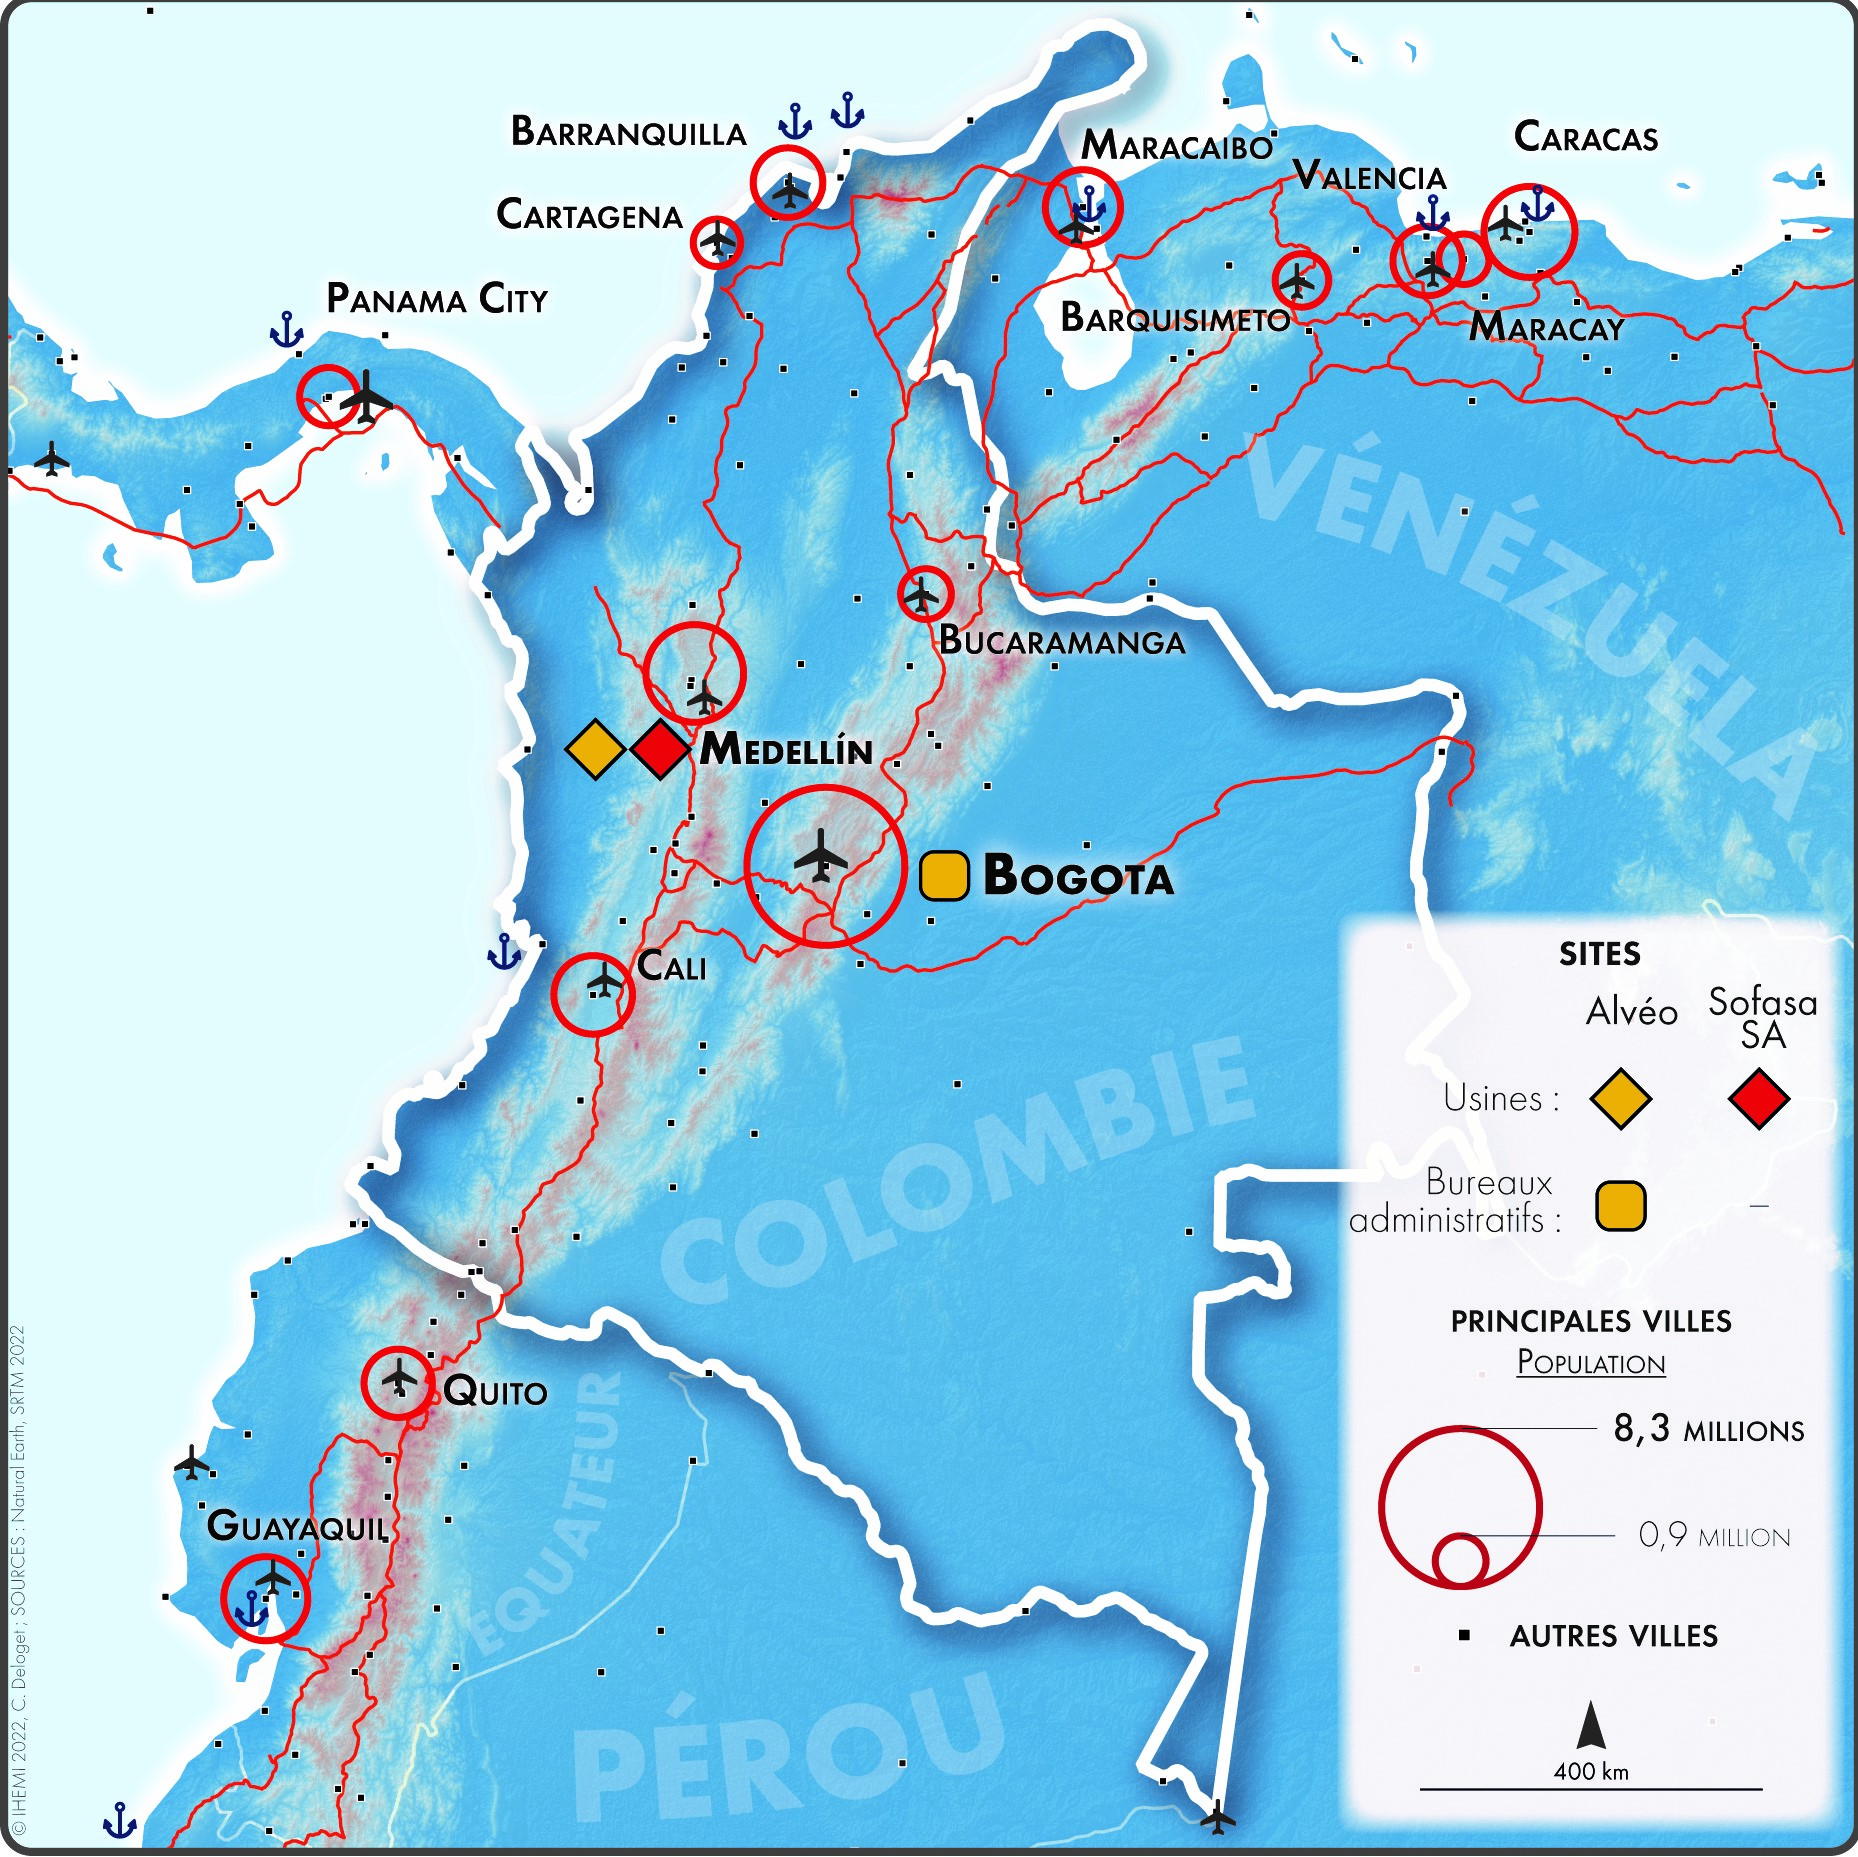
\includegraphics[width=0.8\textwidth]{figures/ALVEO_SituationColombie.jpg}
    \caption{Carte de localisation des locaux d’une entreprise fictive pour le dossier joueurs}
    \label{fig11}
\end{figure}

\begin{figure}[!t]
    \centering
    \includegraphics[width=0.8\textwidth]{figures/reseau_ferre.jpg}
    \caption{Carte du réseau ferroviaire passagers, dans une rubrique transports d’un dossier joueurs}
    \label{fig12}
\end{figure}

Les types de cartes présentées ici sont le résultat de deux de mes missions : assurer le rôle de cartographe lors d’exercices de gestion de crise dans une salle pédagogique et réaliser des cartes associées à la conception des scénarios joués lors de ces mêmes exercices. Elles sont donc le reflet des caractéristiques intrinsèques à une crise gérée par des acteurs institutionnels dans un département : ici, une rencontre directe de différents acteurs publics impliqués dans la crise (que j’ai tenu à présenter longuement au début de cette partie), dans le contexte d’incertitude et de dérobement propre au déclenchement d’une crise. Une crise déclenchée par une équipe d’animateurs et établie dans un scénario. Celui-ci nécessite une préparation et un besoin en cartographie en partie couvert par la seconde mission qui m’était proposée. J’ai commencé à aborder certains points tels que la disponibilité des données et leur représentation. De même que les spécificités liées aux scénarios de crises fictives et par conséquent à la dimension pédagogique des missions du DRC. Je vais maintenant tenter, dans la troisième partie, de présenter une certaine prise de recul sur le travail qui m’a été demandé.


\end{part}



%%---------------------------------TROISIEME PARTIE--------------------------------------


\begin{part}{La réalisation de cartes pour la formation à la gestion de crise : résultats, réflexions et autres enjeux}
Cette troisième partie présente un ensemble de réflexions personnelles concernant à la fois mes réalisations et l’environnement professionnel dans lequel s’est déroulé mon stage. 
    
Je présenterai d’abord certains points d’attention spécifiques aux missions de l’IHEMI et du DRC. Je détaillerai ensuite la manière dont prennent place les données et notamment l’information géographique dans l’ingénierie pédagogique et notamment la création des scénarios. Je présenterai aussi dans ce chapitre l’une de mes réalisations : une ébauche d’outil de visualisation cartographique pour les scénarios utilisant une base de données spatiale. Le dernier chapitre regroupe plusieurs autres réflexions plus générales sur la cartographie en gestion de crises.

\mychapter{4}{Formation à la gestion de crises et place de la cartographie}
La figure ~\ref{fig13} ci-dessous présente les dimensions qui influent, selon moi, sur le type de cartes réalisables dans le contexte de la gestion de crise, avec des exemples dont certains sont issus de réalisations produites durant mon stage. Certaines dimensions ont été pensées en fonction des différents aspects que je détaille maintenant.

\subsubsection{Différentes granularités à cartographier}
J’ai, dès le début du stage lorsque j’étudiais les scénarios de crise pour la réalisation des planches auditeurs format A3, été surpris par l’importance de bien prendre en compte la temporalité de chaque \textit{input}. Sur une planche cartographique statique distribuée à une heure donnée aux auditeurs, on l’a dit, impensable de faire figurer des informations ou des événements futurs. Les scénarios contiennent également plusieurs lignes temporelles parallèles : certains événements sont très localisés temporellement. Leur intensité se manifeste sur un temps très court. Dans ce cas, ils sont aussi généralement très localisés spatialement (exemple : une fusillade sur une place). D’autres événements se produisent plus sur le temps long, de manière moins puissante. Ce sont ceux-ci qui sont souvent plus étalés spatialement. (Une plaine inondée par exemple). On peut ainsi selon moi représenter un épicentre spatial de la crise où seront le plus souvent localisés les événements courts, localisés et forts. Autour se trouveront les événements et informations plus dissolues, longues et étalées spatialement. Ceci participe également à la définition d’un système d’enchaînement et de causalité. L’inondation peut par exemple être la cause d’un événement localisé grave. Ces différentes lignes temporelles reliées les unes aux autres est quelque chose de complexe à rendre compte sur une carte. Les représenter, même de manière simplifiée, sur la carte présentée dans la figure ~\ref{fig9}, par un gradient de couleur et par une frise chronologique a été chose complexe. Dans le cas de carte à destination des joueurs, ceux-ci n’ont accès qu’aux \textit{inputs} qu’ils soient « longs » ou « courts » qui se sont déjà produits. Dans le cas d’une carte qui ne se focalise que sur un ou un groupe d’inputs particuliers (carte localisée souvent pour le pôle communication du COD pour communiquer à l’extérieur de la salle), la temporalité de l’input influence le type de carte alors produite. Il s’agit, sur la figure ~\ref{fig13}, qui présente les variables influençant le type de cartes réalisées, de l’axe appelé « étendue temporelle et spatiale». 

Les animateurs peuvent, eux, avoir, nous l’avons vu, une vision omnisciente, et disposer d’informations fixées et clairement définies, qui sont parfois l’objet d’incertitudes côté joueur durant un certain temps de la crise. On pensera par exemple au nombre de blessés (indiqués UA ou UR sur la carte) ou au nombre de personnes décédées (indiquées DCD sur la carte).

\subsubsection{Le double jeu animateur-joueur}
Cette opposition de point de vue sur les \textit{inputs} entre animateur et joueurs nécessite une précision supplémentaire. En tant que cartographe du DRC placé auprès des joueurs, j’étais à la fois connaisseur du scénario, après quelques exercices, de manière quasi omnisciente. Tout comme l’équipe du DRC qui conçoit les scénarios, je me devais de m’imprégner de ceux-ci, notamment pour la réalisation des planches animateur. Mais la conséquence est que lors des exercices en salle de crise, je pouvais même parfois, hors différences liées à leur profil, anticiper les demandes que les joueurs allaient me faire. Une partie de ma mission consistait alors à ne pas laisser transparaître cette connaissance amont du scénario et à réagir aux demandes, alimenter le support commun et à produire mes cartes comme si je découvrais le scénario, bien que j’anticipais la préparation d’un fond de carte et un ensemble de jeux de données prêts à être affichés à la demande. Il s’agit de faciliter le déroulement et la préparation de l’exercice sans court-circuiter sa conduite en révélant les \textit{inputs} à l’avance. Ce double jeu a parfois été complexe à gérer, surtout dans les premiers temps du stage, et ce double rôle n’était que rarement pleinement cerné par les auditeurs, qui me confondaient parfois, malgré une présentation de l’équipe du DRC avant l’exercice, avec un intervenant extérieur. Et ce, d’autant plus que lorsque j’étais au côté des joueurs, il ne m’était que peu aisé de communiquer avec l’équipe d’animation. Et cette dernière décide du déclenchement des \textit{inputs}. Elle peut, volontairement, ne pas en déclencher certains. Je devais donc, moi aussi, faire face à une certaine incertitude, non pas sur le fond de l’exercice comme cela était le cas pour les auditeurs, mais bel et bien sur sa forme et son déroulement, en plus souvent de la singularité des auditeurs et de leur profil. Le rôle du cartographe est donc dans ce cadre, en plus des particularités et de l’ambiance propres à la salle de crise activée, complexe et non-unique vis-à-vis du public demandeur de cartes et du public lecteur. 

\subsubsection{Interprofessionnalité, demandes de cartes et pédagogie}
Les auditeurs reçus ne sont issus qu’indirectement du milieu de la gestion de crise – que ce soit la sphère privée ou la sphère police-armées. Ajouté au fait qu’ils soient formés à ces procédés et cela mène à deux choses : ils ne sont que peu familiers avec la cartographie et ce ne sera de toute façon, en tant que décideurs, hauts fonctionnaires, gestionnaires de crise, pas leur spécialité. Certains ne sont pas du tout familiers de la discipline. Il arrivait parfois que ma place et mon rôle dans la salle de crise ne soient pas ou que tardivement compris. D’autres auditeurs ont quant à eux connaissance d’outils tels que Maps, le Géoportail, la carte IGN et font partie de ce que j’appelle la « population convaincue ». Ce sont des personnes qui ont une connaissance d’outils grand public et surtout sont convaincue de l’utilité de l’outil cartographique. C’est cette catégorie d’auditeurs qui venait, souvent dès le début de l’exercice me solliciter, tout en étant à l’écoute des suggestions et remarques que je pouvais leur communiquer. Dans la phase la plus critique et la plus incertaine de la crise, je répondais parfois à des questions basiques de type où se trouve tel élément ? Dans l’urgence, solliciter le cartographe se veut rassurant. Au cours de la gestion de crise, le fond de carte présente également des éléments autres que ceux relatifs aux \textit{inputs} : des éléments de contextualisation, préparés en amont sur un fond de carte. 
Mais aussi souvent des éléments demandés par les joueurs en fonction du contexte de l’exercice. Dans ce cadre, j’ai été amené à refuser des demandes soit farfelues soit, surtout, irréalisables, notamment par soucis de manque de pertinence ou d’absence de données. Et cet aspect, même pour les personnes convaincues, est inconnu des auditeurs. Parmi les demandes des plus pertinentes, il m’a par exemple été demandé de faire figurer les zones forestières possiblement inondées dans le cadre de l’exercice se déroulant dans l’estuaire de la Gironde afin de coordonner les décisions prises avec l’ONF. Ou bien, dans un exercice de type accident industriel, la réalisation d’une zone tampon selon un angle et une orientation définie pour figurer la zone située sous un nuage de fumée (une plume). Ces éléments de contexte participent à un premier niveau d’analyse contextuelle de la situation. Ces demandes d’un niveau d’analyse plus élevé émanent souvent d’un public de joueurs formés à des techniques cartographiques liées à leur activité professionnelle. Elles étaient souvent formulées par des Gendarmes, militaires des trois armées ou bien des Sapeurs-Pompiers, qui ont une grande culture cartographique dans le domaine des SIG. Toutefois, ceux-ci sont des professionnels de l’opérationnel tactique. Par conséquent, par déformation professionnelle, ils souhaitent parfois voir figurer sur le support partagé ou sur les productions cartographiques l’emplacement précis, parfois à une dizaine de mètres près, des unités de gendarmerie, des armées ou de sapeurs-pompiers sur les lieux d’un incident présent dans le scénario, sur un support d’emprise régionale. Alors que le support partagé est à vocation stratégique et nécessite une sélection des informations générales et globales dans le but d’une aide à la conscience situationnelle partagée. Dans la même idée, les auditeurs des CCT par exemple, sont eux plus habitués à gérer une crise en COD, et ont par conséquent des attentes et sont très critiques de l’organisation formelle de l’exercice. Il s’agit des auditeurs parmi les plus exigeants et cela appelle à un positionnement de cartographe expert plus assuré.
%figure ~\ref{fig13}
\begin{figure}[!b]
    \centering
    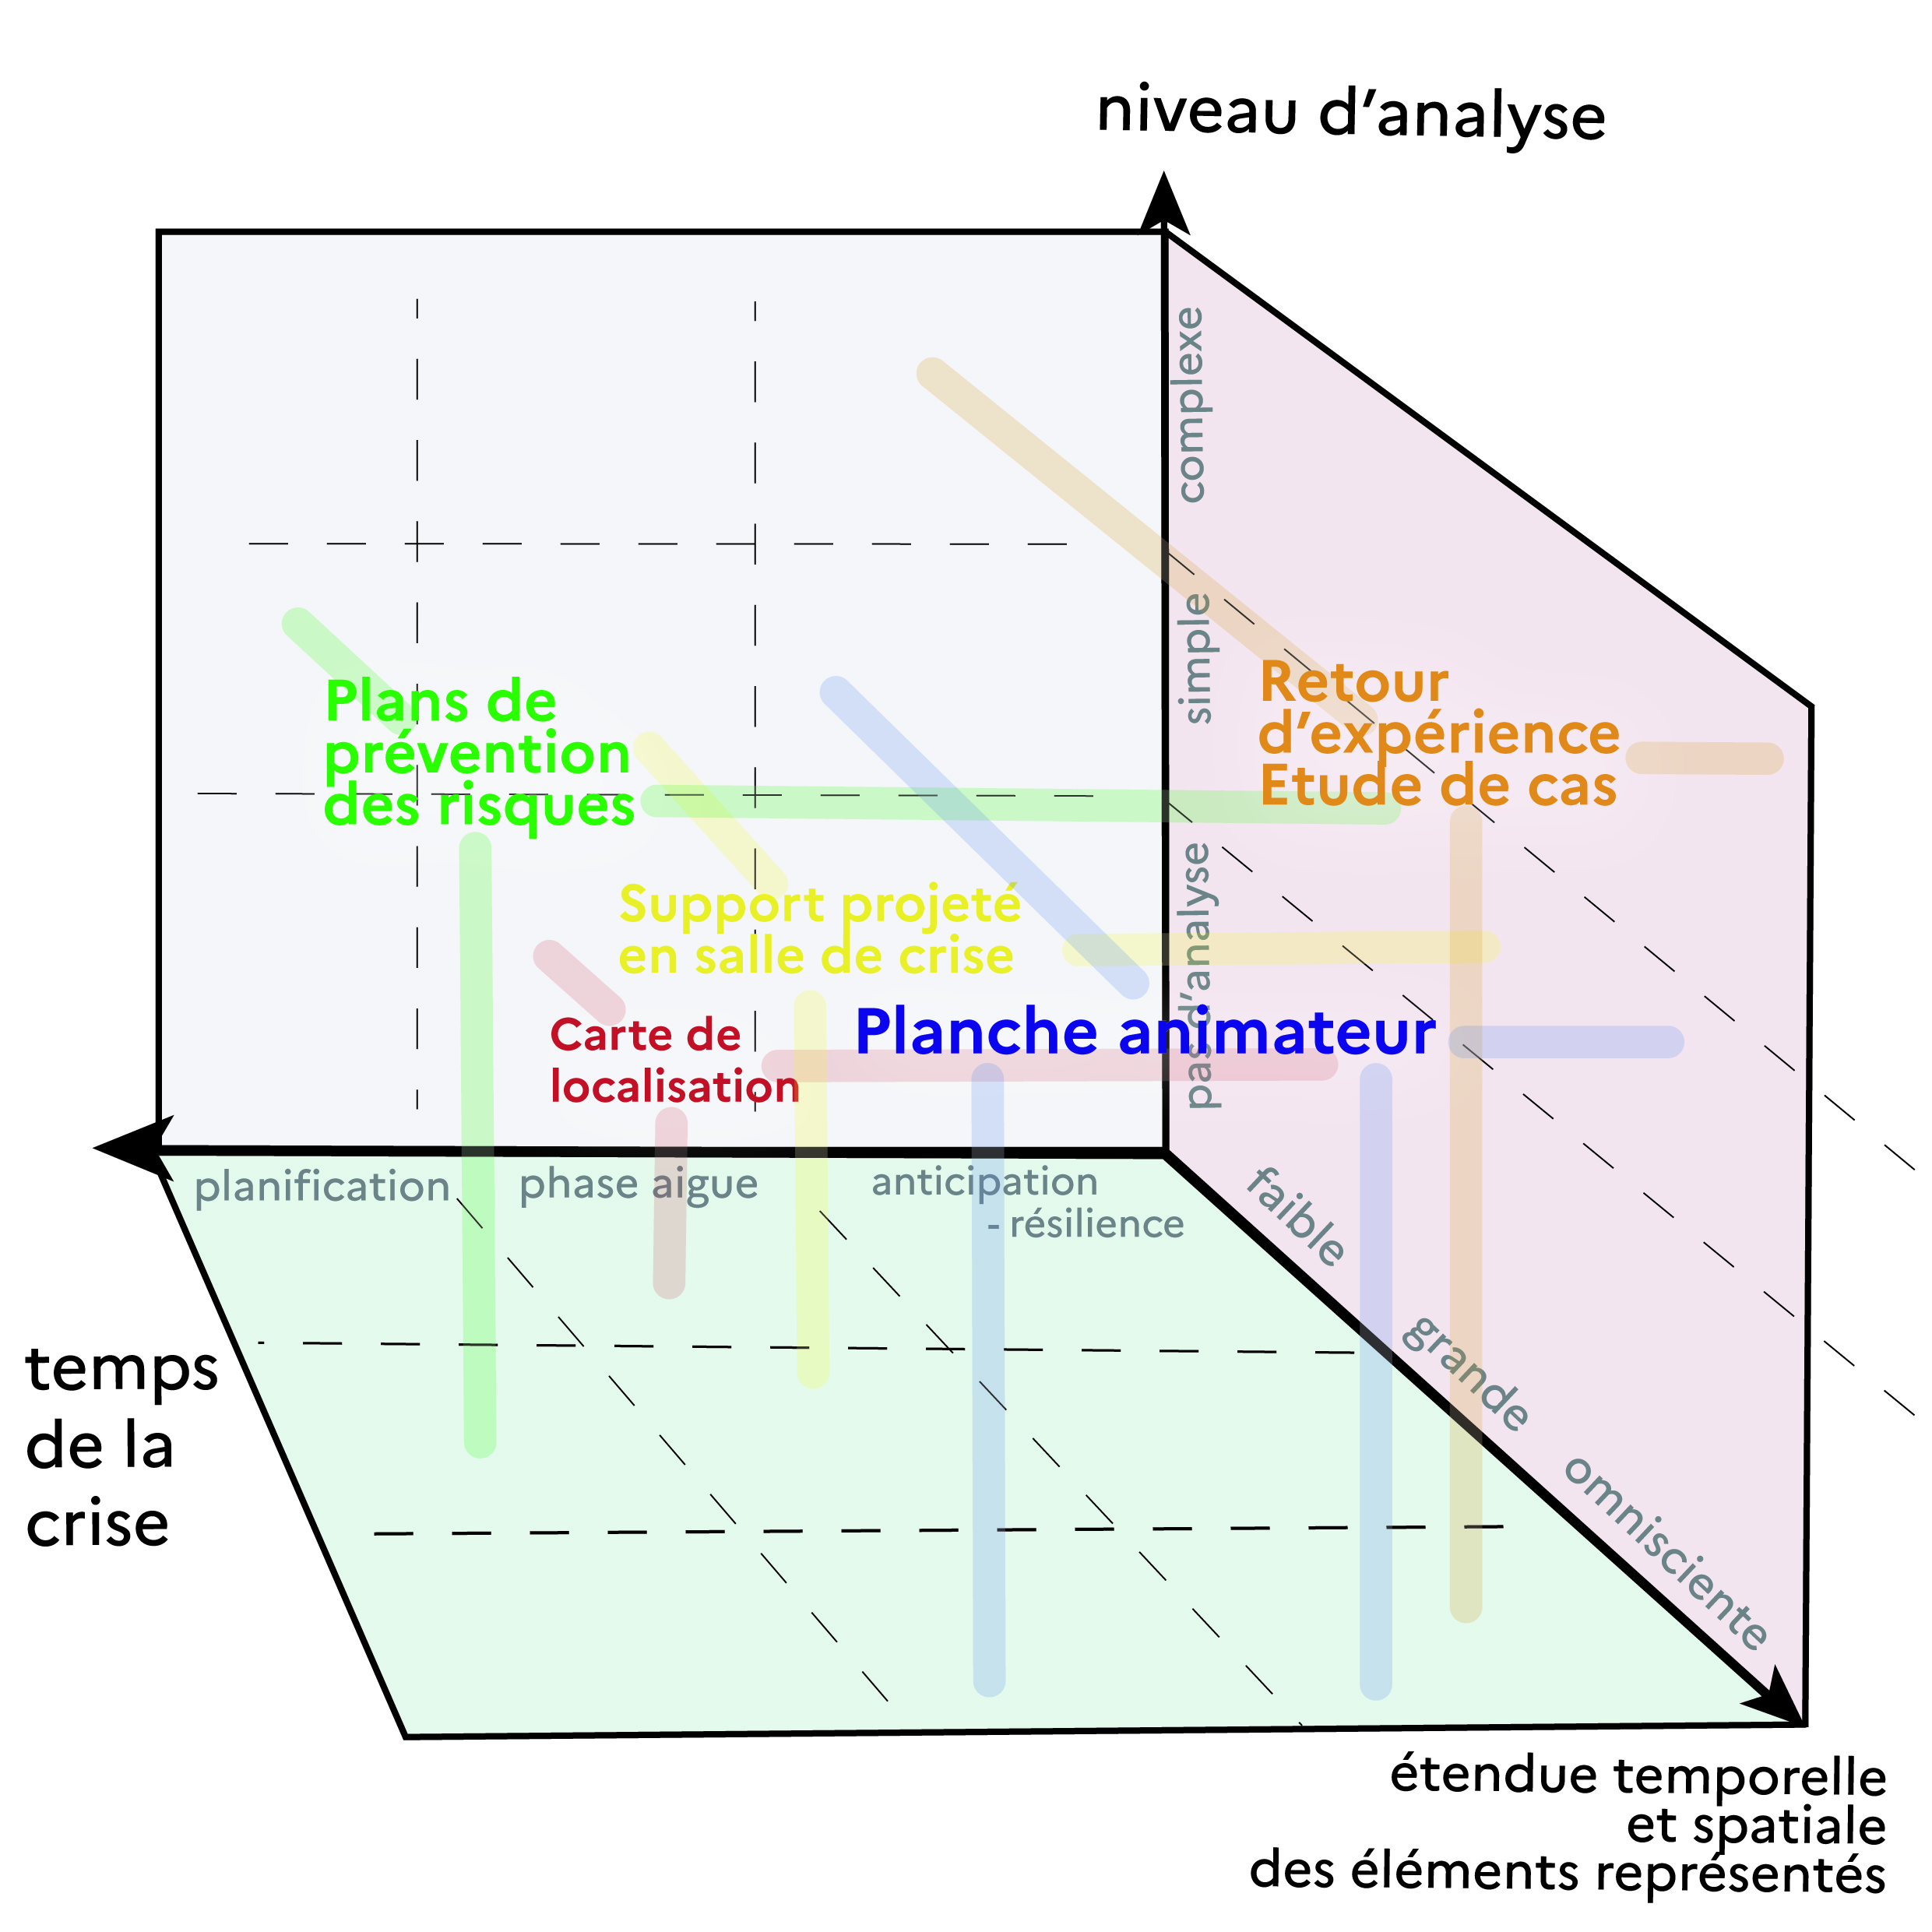
\includegraphics[width=0.8\textwidth]{figures/schema_cube.jpg}
    \caption{tentative de représentation des facteurs influant sur le type de cartes pouvant être produites en gestion de crises}
    \label{fig13}
\end{figure}

\subsubsection{La carte comme vitrine des formations}
La présence d’un cartographe en cellule de crise, ainsi que la présence de support cartographique pour les auditeurs et les intervenants constituant l’équipe animateurs, participent à assurer la légitimité de l’IHEMI et du DRC comme acteur de référence dans la formation à la gestion de crise. Et ce, dans les deux cercles du réseau d’auditeurs : à la fois dans le cercle interne interministériel et à la fois dans les partenaires et auditeurs externes. L’IHEMI et le DRC cherchent à assurer leur positionnement : des cartes de qualité et la présence d’experts tendent à rendre appréciable et qualitative la formation pour les auditeurs.

\mychapter{5}{Culture de la donnée et harmonisation des informations géographiques}
Si les scénarios de crise sont décrits dans un format normalisé dans un tableau Excel, il n’existe pour le DRC aucune bibliothèque ou structure de données géographiques. Ceci peut s’expliquer par deux éléments : l’IHEMI n’est pas une structure spécialisée dans le domaine de l’informatique ou du numérique : elle a été créée par et pour des fonctionnaires du ministère de l’Intérieur, spécialisée dans la sécurité civile ou l’ordre public. De plus, sa création et le regroupement de ses différents départements ne sont que relativement récents. Cela explique, de manière générale, que l’IHEMI n’ait pour l’instant que peu de culture de la donnée informatique, en dehors de l’équipe informatique (le service SIC) bien évidemment. Par exemple, il n’existe aucun document commun qui référence les auditeurs et les intervenants de chaque département et qui soit commun à l’Institut. Si des rétroplannings et des comptes-rendus sont demandés aux agents des différents départements, il n’existe toutefois aucun formalisme commun. Et ceci vaut également pour l’information géographique. Ces points ont par ailleurs été soulignés lors d’un séminaire d’amélioration auquel j’ai participé. Concernant les scénarios, elle est absente. Les seuls jeux de données qui m’ont été fournis l’ont été par un agent du DRC, adjudant de Gendarmerie. Cette démarche a été conduite à titre personnelle, avec des données qu’il avait en sa possession, culture de la cartographie opérationnelle chez les gendarmes oblige.

C’est face à ce constat que j’ai commencé à élaborer un outil de visualisation cartographique des scénarios qui répondrait à deux contraintes. Il était d’ailleurs prévu que je poursuive un travail de développement d’outil débuté par ma prédécesseuse. Cet outil, premièrement, permettrait de prendre en compte les spécificités cartographiques propre à la formation à la gestion de crise. C’est-à-dire la prise en compte de l’opposition joueur-animateur, des différentes temporalités, d’une accessibilité sur plusieurs postes du DRC et l’utilisabilité par un grand public. Deuxièmement, il se baserait sur un schéma de base de données normalisé et évolutif, basé sur l’outil PostgreSQL et son extension spatiale PostGIS. 

La figure ~\ref{fig14} présente un diagramme UML simplifié décrivant la base de données telle que je l’ai élaborée. Celle-ci permet de décrire les différents éléments d’un exercice de crise. Ce dernier se compose d’un scénario. A un scénario sont liés des évènements et des mesures prises. Les mesures prises pourraient d’ailleurs aussi être liées à un évènement. 
%figure ~\ref{fig14}
\begin{figure}[!b]
    \centering
    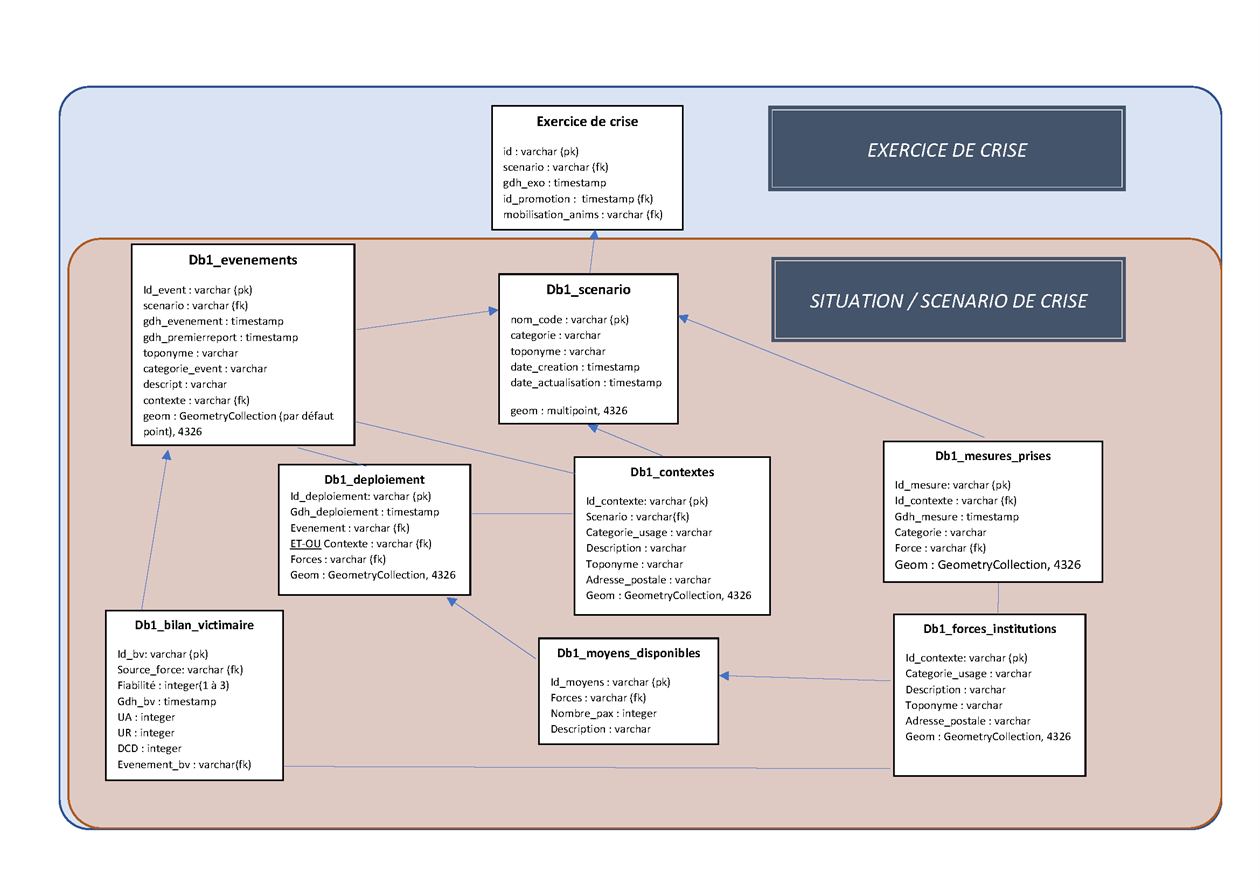
\includegraphics[width=0.95\textwidth]{figures/uml.png}
    \caption{Diagramme UML simplifié d’une proposition de base de données spatiale décrivant les scénarios de crise, source : personnel}
    \label{fig14}
\end{figure}
J’ai ensuite commencé à développer un outil web de visualisation cartographique. Celui se base sur le Framework Node.js comme vu en cours de Cartographie Web durant l’année de Master 2. Celui-ci permet à la fois de mettre en place un serveur web de cartographie dynamique et de se connecter à la base de données pour ensuite les traiter et les proposer sur un serveur sous forme d’une API. Cette possibilité permet d’utiliser les données traitées par le client web sur les pages qui lui sont affichées, mais aussi de les utiliser dans d’autres outils tels qu’un logiciel SIG. L’interface de visualisation cartographique est codée coté client, en javascript, et se base sur la librairie leaflet.js. Le traitement des données requêtées en SQL depuis la base de données est ensuite traité pour être diffusée via une API au format geojson. 

C’est un format à la fois lisible par beaucoup d’outils externes dont QGIS et c’est surtout un format utilisable par la librairie Leaflet. Le script de cet API permettant de requêter les données sur la base et de les traiter pour les mettre en forme en geojson est présenté en annexe 3 . L’ensemble de l’architecture est détaillée dans la figure ~\ref{fig15} ci-dessous. 

Côté client web, l’interface que j’ai commencé à développer permet de choisir entre deux modes : joueurs ou animateur. Ce dernier mode est le seul pour l’instant développé : une interface présente ensuite les scénarios disponibles, reçus via une requête et une API, sur une carte avec une popup qui donne les informations sur le scénario. Si l’utilisateur clique sur l’un des scénarios sont affichés les principaux événements et des informations les concernant sont affichées au survol. Le mode joueur, s’il avait été mené plus loin, comporterait des paramètres (dans l’URL) permettant de fixer un scénario et un groupe horaire qui ne pourrait pas être commodément changé par le joueur. L’ébauche d’interface et les éléments décrits ici sont visibles sur la figure ~\ref{figure:figure}.
%figure ~\ref{fig15}
\begin{figure}[!b]
    \centering
    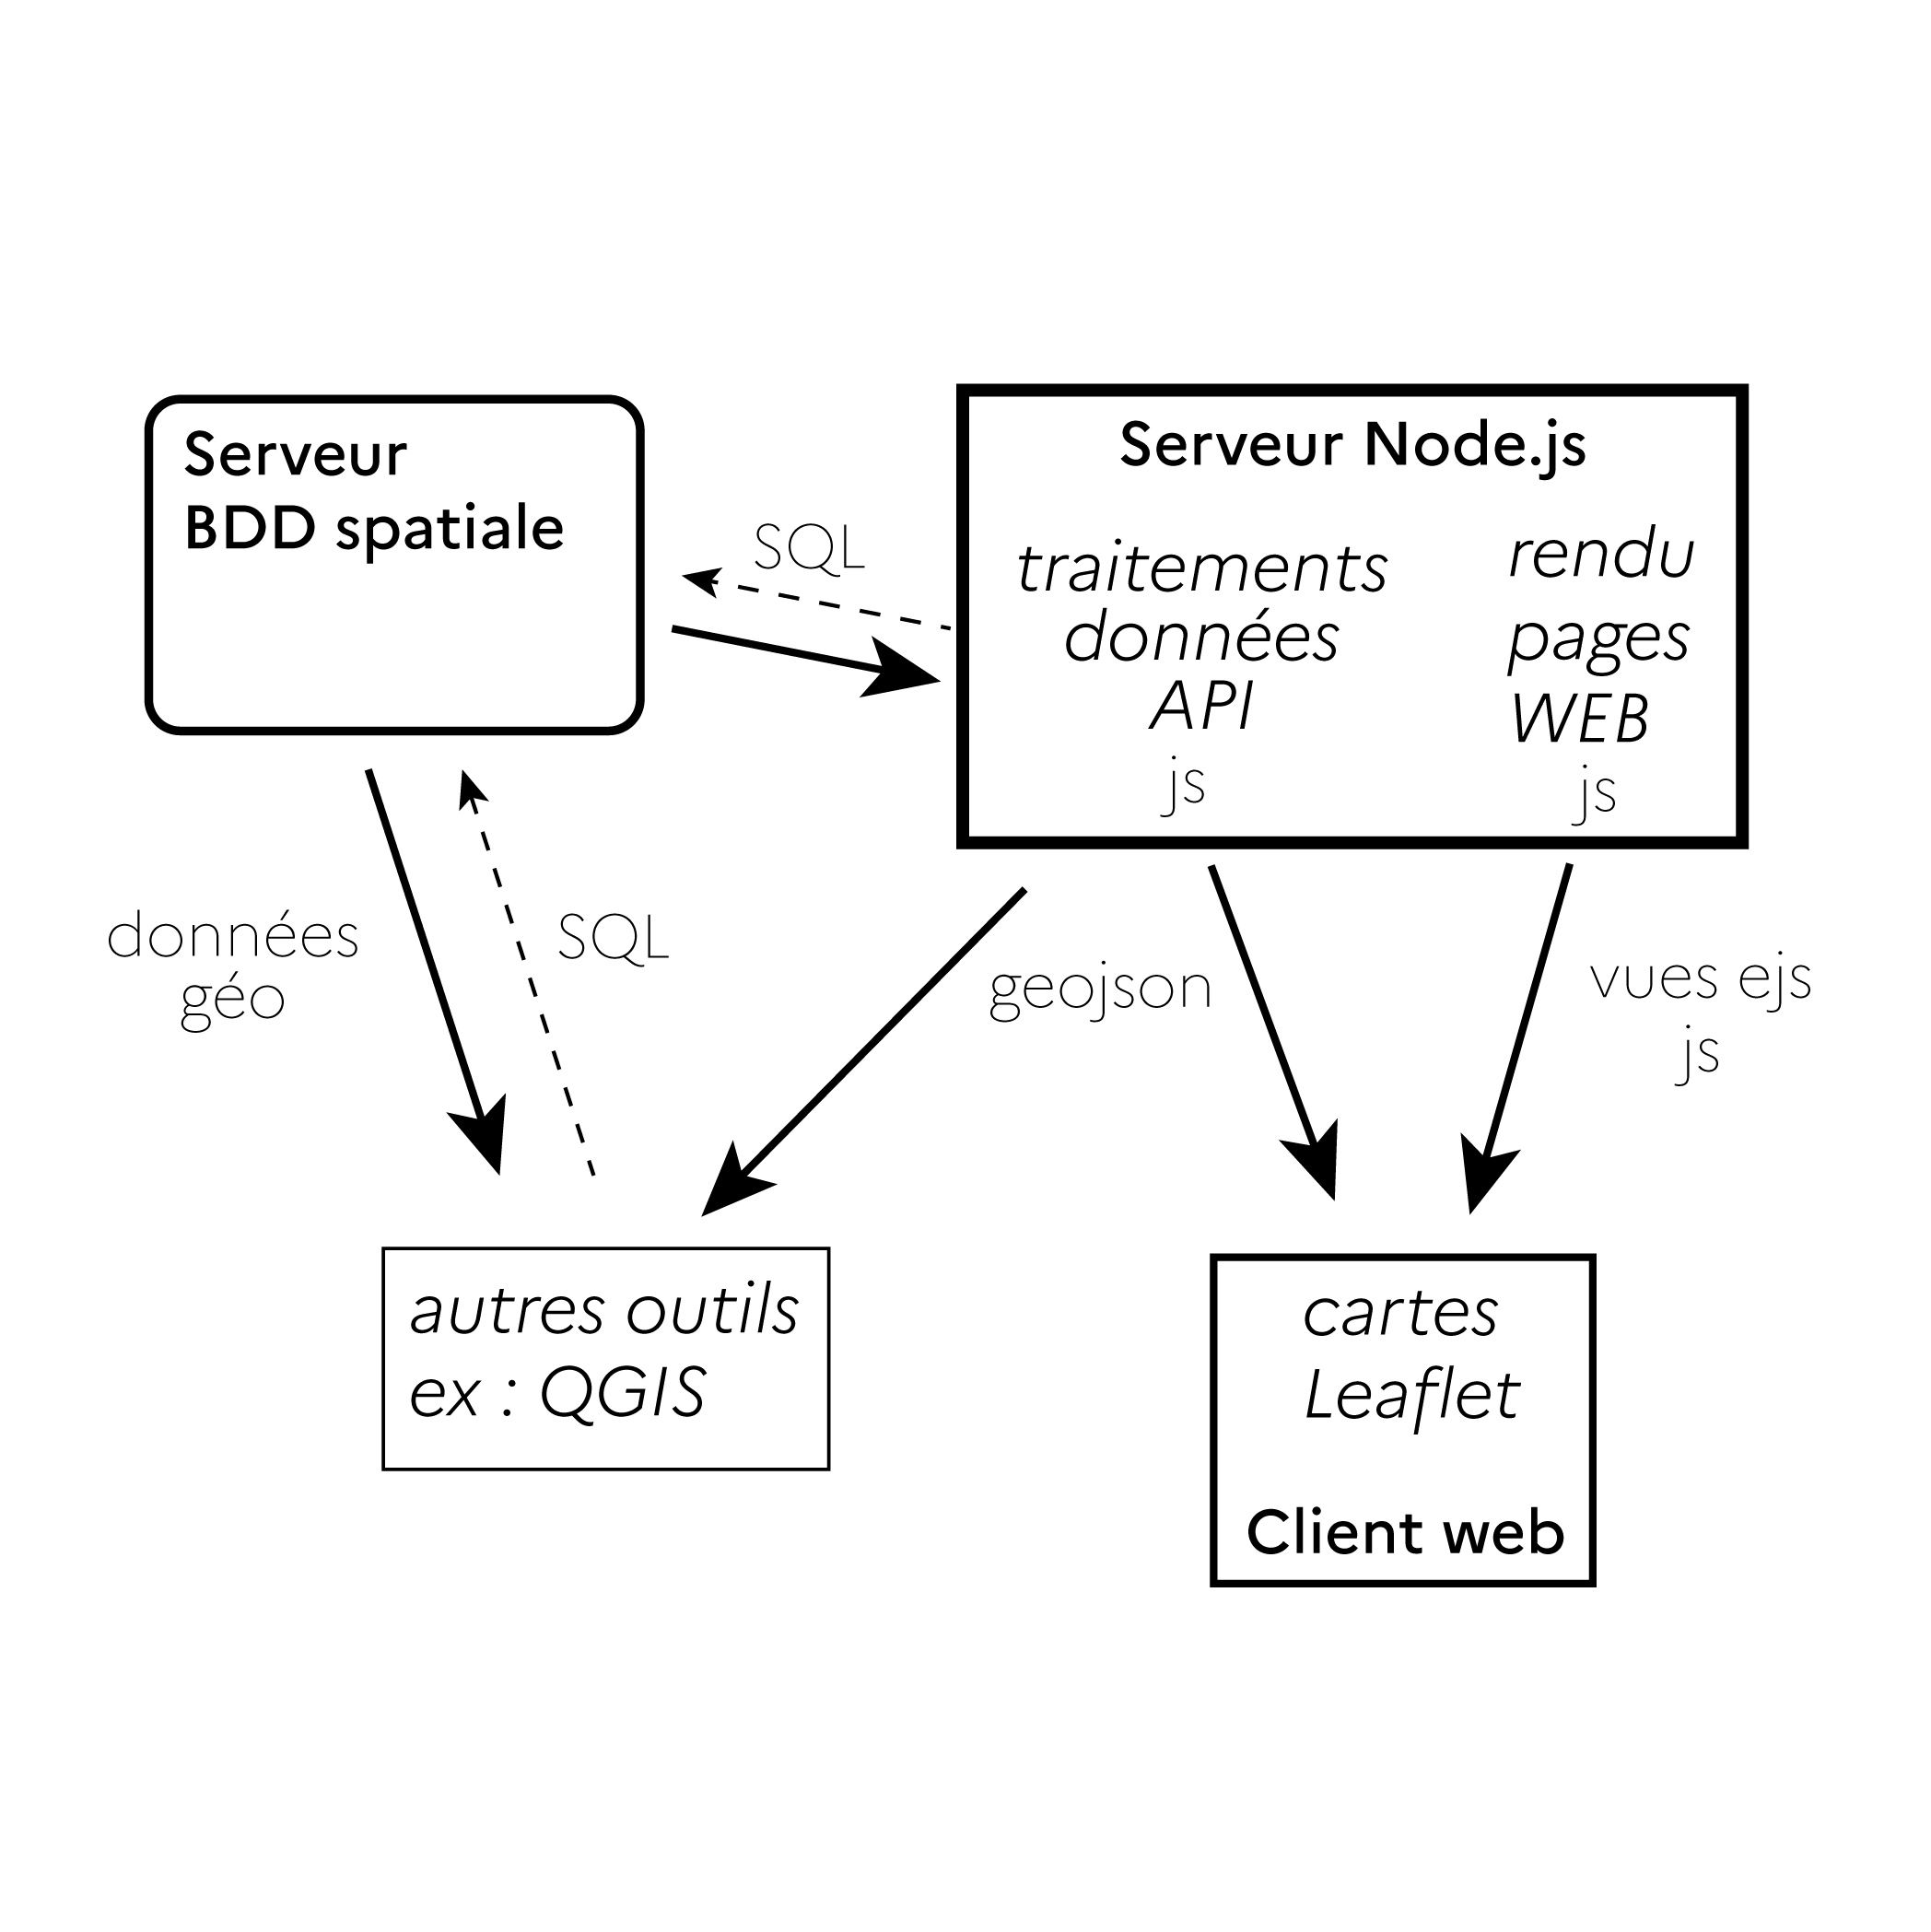
\includegraphics[width=0.7\textwidth]{figures/schema_outil.jpg}
    \caption{schéma de l’architecture de mon outil de visualisation cartographique des scénarios de crise, source : personnel}
    \label{fig15}
\end{figure}

%figure ~\ref{figure:figure}
\begin{figure}[!t]
\begin{subfigure}{\textwidth}
    \centering
    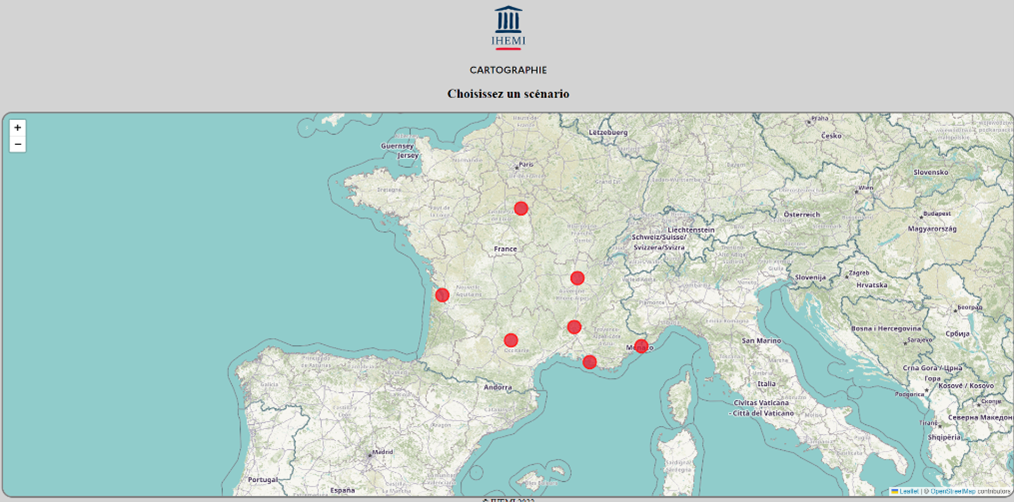
\includegraphics[width=.9\linewidth]{figures/outil1.png}
    \caption{visualisation et choix du scénario}
    \label{figure:sousfig1}
  \end{subfigure}\\
  \begin{subfigure}{\textwidth}
    \centering
    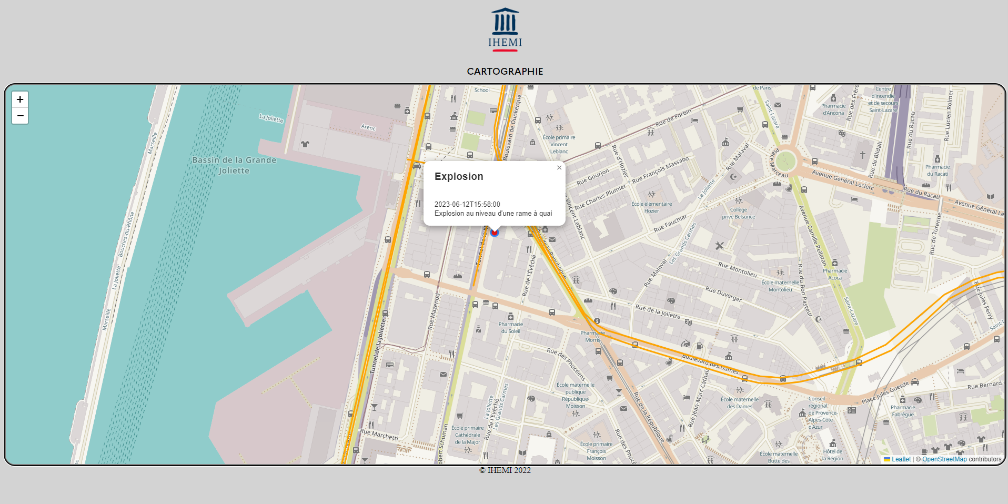
\includegraphics[width=.9\linewidth]{figures/outil2.png}
    \caption{focus sur un événement d'un scénario}
    \label{figure:sousfig2}
  \end{subfigure}
\caption{aperçu de l’ébauche d’interface de visualisation côté client, source : personnel}
\label{figure:figure}
\end{figure}

Cette interface est au stade d’ébauche et a été réalisée sur les dernières semaines de stage parallèlement aux autres missions. Mais j’ai, le plus possible, fait en sorte que les traitements et les fonctionnalités de cette architecture n-tiers soient le plus généralisables possibles. De nouvelles fonctionnalités pourront être développées pour le client selon les besoins et les compétences des personnes qui pourront être impliquées dans le futur sur le projet. Commencer à imaginer cet outil a nécessité un dialogue avec les équipes SIC concernant le déploiement possible de l’outil dans le futur. Le Master 2 Carthagéo, par les notions de gestion de bases de données qu’il dispense me permettait de leur présenter mon projet avec des termes techniques et précis. Mes limites en termes de compétences en développement d’applications se sont néanmoins rapidement fait sentir lorsque les équipes m’ont rappelé leurs contraintes en termes de déploiement d’outils : sécurité des serveurs et compatibilité avec une architecture Linux notamment…

Ceci permet de mieux comprendre la place du cartographe dans une structure comme l’IHEMI : une place d’expert, qui peut dialoguer avec plusieurs champs professionnels : équipes informatique, chargés de missions en gestion de crise et une place de pédagogue pour expliquer les possibilités et présenter des idées en termes d’information géographique et de représentation cartographique.

\mychapter{6}{Un domaine de possibilités}
Cette mission permet de questionner la pertinence des outils de cartographie dans le cadre de la gestion de crise. J’utilisais, à la fois sur le poste de mon bureau et sur le poste de la salle de crise, le logiciel QGIS. Or, si ses nombreuses possibilités et sa polyvalence sont indéniables, notamment au travers des plugins, il comporte plusieurs inconvénients en salle de crise. Premièrement, il n’est pas conçu pour être accessible à un public novice : son utilisation est réservée à un usager cartographe-géomaticien ou de personnes à minima formées rapidement à son usage et aux principes élémentaires de l’information géographique. De plus, il s’agit d’un outil généraliste et non d’un outil « métier » : ses fonctionnalités ne sont pas prévues pour être utilisées dans un délai très court dans un contexte de gestion de crise. Pour adapter son interface et pour optimiser l’enchaînement de géo-traitements, il serait tout à fait pertinent de développer des plugins spécifiques. Ce logiciel SIG est néanmoins très adapté dans les autres temps de la crise, dans les phases de planification et de résilience.

Face à ces deux constats, des outils ont été développés, notamment sous le pilotage de la DGSCGC (ministère de l’intérieur) mais aussi par le Ministère de la transition Ecologique (MTE). L’outil Synapse est par exemple disponible dans un grand nombre de préfecture. Il regroupe des cartes d’aléas, des données concernant les enjeux (sites sensibles type SEVESO, zones peuplées, lignes H.T. etc) et propose quelques géo-traitements typiques (simuler le territoire couvert par une inondation à hauteur donnée, donner le nombre d’habitants présent dans un périmètre etc.).

Il permet de résoudre ainsi un des problèmes évoqués précédemment : la mise à disposition de données harmonisées. Toutefois, il s’agit d’un outil fermé : à l’opposé d’un logiciel SIG où il est possible de développer des modules, Synapse de permet pas de coder de nouveaux traitements, et ses fonctionnalités sont limitées. C’est toutefois un bon compromis pour des personnes non-spécialistes mais ayant besoin d’utiliser un outil d’analyse simple, rapide à prendre en main et toute de même développé spécifiquement.
%figure ~\ref{fig17}
\begin{figure}[!t]
    \centering
    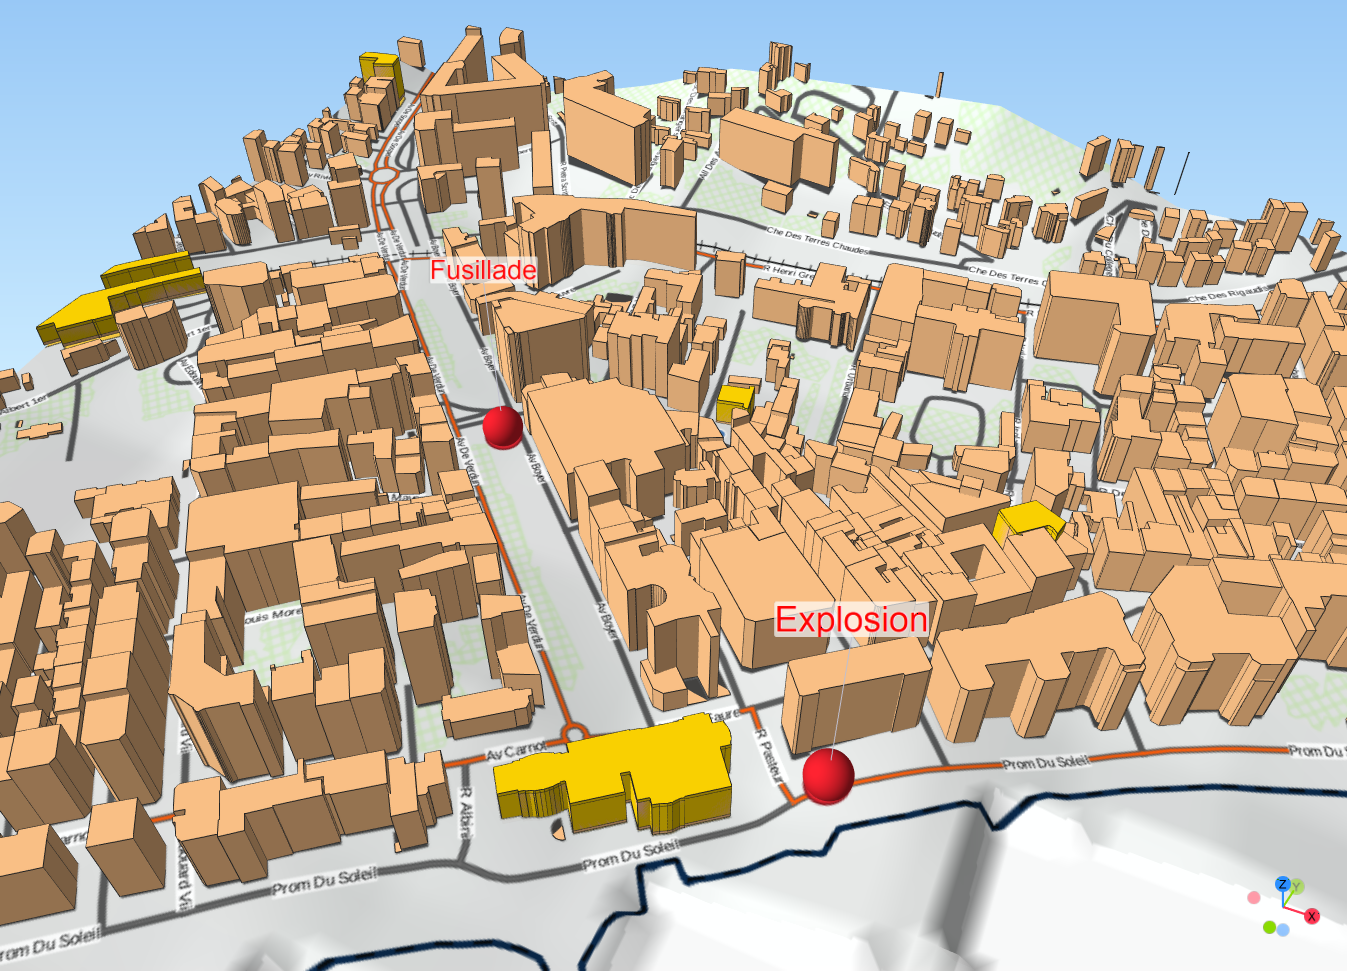
\includegraphics[width=0.95\textwidth]{figures/Menton_local.png}
    \caption{essai d’une visualisation 3D de deux événements fictifs dans la ville de Menton}
    \label{fig17}
\end{figure}
Je terminerai cette partie en évoquant rapidement les possibilités offertes par des représentations innovantes telles que les cartes interactives en trois dimensions. 

Ces dernières me semblent particulièrement pertinentes à une grande échelle (faible étendue spatiale) et dans une temporalité courte, pour comprendre les enjeux directs autours d’un événement localisé. La figure ~\ref{fig17} montre une tentative de réalisation d’une carte de ce type à l’aide du plugin QGIS qgis2three symbolisant une fusillade et une explosion sur le front de mer à Menton. Cette idée est issue de nombreuses demandes d’auditeurs de pouvoir visualiser, notamment grâce à Google Maps, l’environnement proche d’un événement et de comprendre comment est agencé le bâti. Ici, le drapage rend l’immersion moins convaincante, mais c’est bien une plus grande immersion qui est recherchée. Enfin, ce type de représentation, au-delà d’une volonté de représentation fidèle de la réalité, permet de co-visualiser des données complexes et de nature différentes, telles que des prévisions météo, dont les résultats sont issus de simulations.\footcite[Voir les travaux de l'équipe GEOVIS de l'UMR LASTIG. Par exemple][ ]{perrinVisualAnalysisInconsistencies2021}

Les spécificités de la formation à la gestion de crises font naître, un ensemble de particularités et de points d’attention dans la réalisation des cartes qui m’ont été demandées : temporalités diverses dans la crise et dans les \textit{inputs}, niveaux d’analyses différents, le tout dépendant de facteurs internes propres à une salle de crise et d’autres externes, propres à la dimension pédagogique et aux méthodes de travail de l’IHEMI.



\end{part}


%%------------------------Conclusion-------------------------
\part{Conclusion générale}

La réalisation de ce stage au sein du Département Risques et Crises au sein de l’IHEMI a constitué, à titre personnel, une découverte riche d’un milieu professionnel qui m’était quasiment inconnu. En plus du positionnement propre à l’IHEMI, son Département Risques et Crises porte ses missions et ses compétences dans un domaine bien spécifique : la formation à la gestion de crises. Si des acteurs privés existent aussi dans ce domaine, il s’agit de la seule équipe d’un organisme public, au niveau interministériel, à assurer cette mission. Ce caractère interprofessionnel y est, à mon sens, vecteur d’une grande richesse dans le travail réalisé par les équipes, au sein desquelles chacun travaille en bonne intelligence, avec engagement et volonté de faire gagner en qualité les formations dispensées à un public de haut niveau, exigeant et curieux. C’est dans ce contexte que j’ai été intégré à l’équipe du Département Risques et Crises. J’ai rapidement pu découvrir la conduite des exercices de gestion de crises dans une salle pédagogique configurée comme le Centre Opérationnel Départemental d’une préfecture. 

La description de ce contexte, auquel est consacré une large partie de ce rapport, est cruciale pour comprendre les missions qui m’ont été demandées ainsi que l’origine et les particularités de mes différentes réalisations. Ces dernières viennent appuyer la richesse documentaire des scénarios de crise, participe à leur bon déroulement surtout du côté des animateurs de l’exercice. Elle rend de plus, lorsque je suis en salle de crise avec les auditeurs, l’exercice plus riche, plus crédible, et participe à la formation des auditeurs aux spécificités, acteurs et procédés de la gestion de crises par l’État. 

J’ai pu, pour ces différents types de réalisations, mettre pleinement à profit les savoirs acquis au cours de l’année de Master 2 Carthagéo, à la fois en ce qui concerne la maîtrise d’un SIG, les principes de sémiologie graphique, le travail graphique à l’aide d’un logiciel de DAO ou bien la conception et gestion de bases de données relationnelles spatiales. L’équipe du DRC - pleinement convaincue de l’intérêt de la cartographie et pour certains effectifs formés à des outils métiers spécifiques notamment dans la sécurité civile et aux armées - m’a entièrement fait confiance et a été très à l’écoute des remarques et propositions que j’ai pu formuler, notamment sur la conception d’une base de données ou sur l’utilisation de certains outils ou de certaines représentations. L’IHEMI et son DRC est un lieu, s’il reste fortement lié aux champs de compétences du ministère de l’Intérieur, qui est caractérisé par la rencontre de différents corps de métiers, travaillant ensemble en bonne intelligence. Il aurait été souhaitable de pouvoir dialoguer avec d’autres cartographes afin d’approfondir certains savoirs et savoir-faire dans mon domaine de formation. Beaucoup d’aspects techniques abordés en cours ont suscité mon intérêt : j’aurais souhaité pouvoir discuter avec une équipe de cartographe par exemple, d’autres manières de travailler dans cet environnement.

Néanmoins, cette interprofessionnalité, cette variété de profils riches m’a permis d’appréhender le fonctionnement institutionnel de la gestion de crise et de comprendre comment la cartographie et le cartographe y prennent place, mais surtout quel rôle ils ont à y jouer. Elle est aussi la raison pour laquelle les savoir-faire du cartographe sont reconnus et demandés. Il y est donc présent en tant qu’expert, parmi une équipe pluridisciplinaire. C’est un contexte de réalisation de cartes à la fois peu connu, à titre personnel totalement nouveau et peu abordé en cours. Ce rôle nécessite une adaptation certaine lorsque l’on découvre, en stage, un environnement professionnel. Le rôle du cartographe est par ailleurs amené à évoluer, et sa place dans le domaine de la gestion de crises est à mon sens vouée à se consolider, à se formaliser et à apporter de nouveaux types et outils de représentations cartographiques.

Ce stage a représenté une opportunité réelle, en plus d’une découverte d’un champ professionnel, d’améliorer un ensemble de savoirs-être professionnels personnels et vient à ce titre, parfaitement compléter à la fois une première expérience professionnelle mais aussi les enseignements techniques et théoriques abordés dans mon parcours.


\newpage
\thispagestyle{empty}
\mbox{}
\newpage

%%------------------------Remerciements----------------------
\part{Éléments complémentaires}

\mychapter{8}{Remerciements}

Mes sincères remerciements à Mme Anne-Lise Cœur-Bizot, ma tutrice de stage et directrice du Département Risques et Crises, pour m’avoir pleinement accueilli dans son équipe et pour m’avoir fait confiance.

Merci à M. Adrien Van Hamme, maître de conférences associé, pour son accompagnement au cours de mon stage. Merci également à l’ensemble de l’équipe pédagogique.

Il m’est impossible de ne pas remercier l’équipe du Département Risques et Crises. 
Merci au CDT Frédéric Portet pour sa bonne humeur, la passion pour son métier et pour sa volonté d’accompagner, de former et d’intégrer les jeunes stagiaires du DRC. 
Je n’oublierai pas non plus Clara Le Bris, pour nos discussions, pour ses conseils de pro et ses photos. Un grand merci à Erika Luzzato pour ses demandes de cartes, ses propres cartes de grande qualité d’ailleurs, son investissement et sa bonne humeur ; 
à Romain Tosello, aussi pour sa bonne humeur et pour sa maîtrise parfaite de la culture italienne ; à l’ADJ Olivier Delmas pour nos discussions sur son parcours de gendarme, ses conseils et son engagement. 
Bref, à toute équipe du DRC et à tous ceux qui m’ont – directement ou pas – apporté leur aide durant mon stage. 
Un grand merci également à l’équipe SIC pour leur sympathie, leur réactivité, pour m’avoir fourni du matériel informatique au-delà de toute espérance.

Un grand merci et beaucoup de courage pour la suite à tous les autres stagiaires et alternants que j’ai pu croiser : Amélie, Faustine, Eugénie, Lauriane, Victoire...

Merci à mes camarades du Master Carthagéo, particulièrement à ceux de la 413 qui se reconnaîtront et qui m’ont permis de partager idées, inquiétudes, réflexions. A nos échanges radicalement riches ou farfelus selon les moments.

%%--------------------Bibliographie-----------------------------------
\nocite{*}
\printbibliography[heading=bibintoc, title=Bibliographie]

\newpage

%%----------Acronymes rencontrés dans le corps de texte------------
\mychapter{9}{Acronymes}       

IHEMI : \textit{Institut des Hautes Études du ministère de l’Intérieur}


MININT : \textit{Ministère de l’Intérieur}


MDS : \textit{Ministère des Solidarités et de la Santé}


CHEMI : \textit{Centre des Hautes Études du ministère de l’Intérieur}


INEHSJ : \textit{Institut National des Hautes Études de Sécurité et de Justice}


SDIS : \textit{Service Départemental d’Incendie et de Secours}


ENM : \textit{École Nationale de la Magistrature}


INSP : \textit{Institut National du Service Public}


DGGN : \textit{Direction Générale de la Gendarmerie Nationale}


DDSP : \textit{Direction Départementale de la Sécurité Publique}


PTS : \textit{Police Technique et Scientifique}


BRI : \textit{Brigade de recherche et d'Intervention}


DMD : \textit{Délégué / Délégation Militaire Départemental(e)}


BSPP : \textit{Brigade de Sapeurs-Pompiers de Paris}


BMPM : \textit{Bataillon de Marins Pompiers de Marseille}


RETEX / REX : \textit{Retour d’expérience}


ORSEC : \textit{Organisation de la Réponse de Sécurité Civile}


OPJ : \textit{Officier de Police Judiciaire}


DDT : \textit{Direction Départementale des Territoires}


ASN : \textit{Autorité de Sureté Nucléaire}


ANSSI : \textit{Agence nationale de Sécurité des Systèmes d’Information}


CORRUSS : \textit{Centre Opérationnel de Régulation et de Réponse aux Urgences Sanitaires et Sociales}


ARS : \textit{Agence Régionale de Santé}


SIDPC : \textit{Service Interministériel de Défense et de Protections civiles}


MNT : \textit{Modèle Numérique de Terrain}


UA : \textit{Urgence absolue}


UR : \textit{Urgence relative}

\newpage

%----------------table des figures-----------
\listoffigures

%%------------------Annexes-----------------
\begin{appendices} %gestion des annexes
    \addappheadtotoc %ajout de l'entrée annexe à la table des matières

    \appendixpage %ajout d'une partie annexe en fin de doc
    
    %%annexes
    \section{Diagramme de Gantt : rétroplanning approximatif de mes missions}
    \begin{center}
        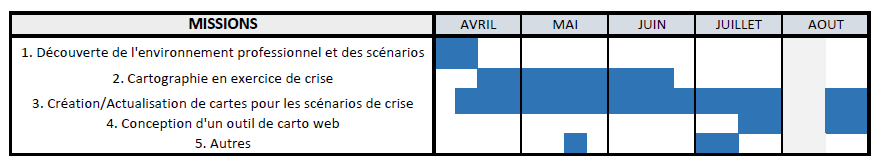
\includegraphics[angle = 90, ]{gantt.png}
    \end{center}

    \section{Adaptation d’une planche animateur au format A0, affichée en salle animateur}
    \begin{center}
        \includegraphics[width = 0.95\textwidth]{plancheA0.jpg}
    \end{center}
    \newpage
    \section{Code javascript d'une des API réalisées}   
    \begin{verbatim}
        //APi qui renvoie les caractéristiques des scénarios dispos 
        //(et pas seulement les noms), 
        //notamment pour affichage de la première carte, 
        //au format geojson

app.get("/api/listerscenario", function(request, response){ 
    //ecoute d'une requete get 

    let marequete = `SELECT ST_AsGeoJSON(t.*)::json
    FROM "db1_scenario" 
    AS t`; //requete permettant de mettre en forme 
    //le resultat en geojson

    marequete = `SELECT json_build_object(
        'type', 'Feature',
        'features', json_agg(ST_AsGeoJSON(t.*)::json)) 
        FROM "db1_scenario" AS t`;

    console.log(marequete);
    pool.query(marequete, [], (error, results) => { 
        //requete sur la table qui liste les scenarios
        if (error) {
            response.send("API : erreur lors de la requête") 
            //si erreur, on envoie le texte suivant au client
        } else {//si pas d'erreur

        response.send(results.rows[0].json_build_object.features); 
        //on envoie le geojson au client
    }});
});

    \end{verbatim}

    \newpage
    \section{Cahier des charges de l’outil web de visualisation cartographique, rédigé en fin de stage}
    \includepdf[pages=-]{cdc_cartoweb.pdf}


\end{appendices}
\newpage

\newpage
\thispagestyle{empty}
\mbox{}
\newpage

\end{document}                        % fermeture d'un environnement